%!TEX program = xelatex
\documentclass[a4paper,12pt,openany,twoside]{book} % twoside
\usepackage[inner=3.5cm,outer=2.5cm, top=2.5cm]{geometry} %showframe

\usepackage{url}
\usepackage{fontspec}
\usepackage{lmodern}
\usepackage{csquotes}
\usepackage{graphicx}
\usepackage{caption}
\usepackage{subcaption}
\usepackage[rgb]{xcolor}
\graphicspath{ {assets/} }
\usepackage{xunicode}
\usepackage{xltxtra}
\usepackage{chngcntr}
\usepackage[czech]{babel}
\usepackage[pagestyles,medium]{titlesec}
\usepackage{setspace}
\usepackage{emptypage}
\usepackage{xpatch}
\usepackage{caption}
\usepackage{subcaption}
\usepackage{ragged2e}
\usepackage{pbox}
\usepackage{rotating}
\usepackage{float}
\usepackage{afterpage}
\usepackage{tipa}

\usepackage[hidelinks]{hyperref}

\usepackage{mdframed}
\usepackage{framed}
\def\tightlist{}

\xpatchcmd{\part}{\thispagestyle{plain}}{\thispagestyle{empty}}{}{}


\newcommand\exmp{\textsf}

\counterwithout{figure}{chapter}
\counterwithout{footnote}{chapter}


\newpagestyle{sensible}{
	\headrule\sethead{}{}{\MakeUppercase{\chaptertitle}}
	\setfoot{}{\thepage}{}
}

\setlength\emergencystretch{1em}
\setlength\headheight{14pt}
\setstretch{1.1}
\setcounter{secnumdepth}{4}

\widowpenalty10000
\clubpenalty10000

\hyphenation{выпа-дений}

\setmainfont[Ligatures=TeX]{CMU Serif Roman}

\usepackage[backend=biber, style=iso-authoryear, sortlocale=cs\_CZ, uniquelist=false, autocite=footnote, maxcitenames=2, maxbibnames=99, minnames=1, urldate=long, spacecolon=false,bibencoding=UTF8
]{biblatex}
\let\oldmultinamedelim\multinamedelim
\let\oldfinalnamedelim\finalnamedelim
\renewcommand*{\multinamedelim}{~a~}
\renewcommand*{\finalnamedelim}{~a~}
\renewcommand*{\nameyeardelim}{~}
\AtBeginBibliography{%
  \renewcommand*{\multinamedelim}{~--\space}%
  \renewcommand*{\finalnamedelim}{~--\space}%
}
\DefineBibliographyStrings{czech}{%
  mathesis = {Bakalářská diplomová práce},
  editors = {eds.}
}

\addbibresource{bibliography.bib}

\newcommand{\sign}[1]{%      
  \begin{tabular}[t]{@{}r@{}}
  \makebox[2.5in]{\dotfill}\\
  \strut#1\strut
  \end{tabular}%
}


\begin{document}
	\clearpage
	\pagenumbering{gobble}

	\begin{titlepage}
		\begin{center}
			{\Large\uppercase{Masarykova univerzita}}

			\vspace{1em}

			{\Large Filozofická fakulta}

			\vspace{1em}

			{\large Ústav českého jazyka}

			\vspace{1em}

			{\large Český jazyk se specializací počítačová lingvistika}

			\vspace{11em}

			{\large Kryštof Davídek }
			
			\vspace{3em}
			
			{\LARGE\bf Elektronický slovník s definicemi založenými na derivačních rysech slovotvorně motivovaných slov}

			\vspace{1.5em}

			{\Large Bakalářská diplomová práce}

			\vfill
			\vspace{3em}
			Vedoucí práce: Mgr. Adriana Válková
			
			2019
		\end{center}
	\end{titlepage}


\cleardoublepage

\par
\par\vspace*{\fill}
	\pagestyle{plain}
\pagenumbering{roman}
\begin{flushright}
	Prohlašuji, že jsem bakalářskou diplomovou práci vypracoval samostatně s~využitím uvedených pramenů a~literatury.

	\vspace{3em}

	    \makebox[2.5in][r]{\dotfill}
	    
	    Kryštof Davídek

	    \par

\end{flushright}
\clearpage

\par
\par\vspace*{\fill}

Na tomto místě bych rád poděkoval své vedoucí práce Adrianě Válkové za veškeré rady a poznatky, které mi ochotně poskytovala po celou dobu psaní této práce.

\clearpage

\section*{Abstrakt}
  
Předkládaná bakalářská práce si klade za cíl navrhnout mobilní aplikaci, jež umožňuje využívat derivačních rysů při osvojování češtiny jako druhého jazyka. Aplikace má podobu elektronického slovníku, v němž jsou definice založeny na strukturním významu slovotvorně motivovaných slov. Pro vytváření slovotvorných definic jsou využita volně přístupná data z derivační sítě DeriNet a pro vývoj aplikace byl zvolen framework Ionic.

\section*{Abstract}

The aim of this bachelor thesis is to design a mobile application that enables to use the derivation features in acquiring Czech as a second language. The application is in the form of an electronic dictionary in which definitions are based on the structural meaning of motivated words. For creating word-forming definitions, freely accessible data of the derivation network DeriNet are used and the Ionic framework was chosen for application development.

\section*{Klíčová slova}

slovotvorba, derivace, derivační morfologie, mobilní aplikace, DeriNet, Ionic, Angular

\section*{Keywords}

word formation, derivation, derivational morpohology, mobile application, DeriNet, Ionic, Angular

\clearpage

\tableofcontents


\cleardoublepage
\pagenumbering{gobble}

% \newgeometry{top=2.5cm}

\pagenumbering{arabic}
\hypertarget{uxfavod}{%
\chapter*{Úvod}\label{uvod}\addcontentsline{toc}{chapter}{Úvod}}

Derivace v~užším smyslu představuje v~českém jazyce, jakožto v~jazyce
s~vysoce rozvinutou flexí, nejčastější způsob utváření nových pojmenování.
Její podstata je nejčastěji založena na přidávání slovotvorného morfému
před (prefix) anebo za (sufix) slovní tvar. Rodilí mluvčí podvědomě
chápou sémantiku jednotlivých morfémů, a~proto si jsou schopni nejen
vyložit významy slov, které v~dané podobě nikdy neslyšeli, ale taktéž
takové novotvary vytvářet. U~cizinců učících se češtinu si je však
potřeba sémantiku těchto odvozovacích prostředků nejprve vědomě osvojit.
V~současné době neexistuje nástroj, který by byl určen pro účely
osvojování derivačních prostředků češtiny.

Cílem této práce je navrhnout a~implementovat elektronický slovník
s~definicemi založenými na derivačních rysech slovotvorně motivovaných
slov. Výsledná aplikace provádí pro zadaný vstup částečnou slovotvornou
analýzu, na základě které zadanému slovu přiřazuje definici vycházející
z~jeho struktury (potažmo strukturního významu).

Teoretickým východiskem pro vývoj aplikace je onomaziologická teorie
slovotvorby představovaná Milošem Dokulilem. Aplikace pracuje s~volně
přístupnými daty derivační sítě DeriNet, jež rovněž vychází z~Dokulilové
teorie. Za využití moderních hybridních technologií pak tato data
zpracovává formou mobilní aplikace.

Práce se skládá ze dvou částí -- teoretické a~praktické. V~teoretické
části jsou nastíněny synchronní přístupy k~české slovotvorbě a~současně
je zde hlouběji popsaná onomaziologická teorie slovotvorby. Dále jsou
zde představeny již existující softwarové nástroje, které s~českou
slovotvorbou pracují.

Praktická část se soustřeďuje na popis výsledného nástroje -- nejprve je
představen proces vytváření slovotvorných definic (spolu s~popisem
zpracovaných slovotvorných sufixů) a~posléze je nástroj popsán
z~hlediska jeho návrhu a~implementace.

\part{Teoretická část}

\hypertarget{slovotvorba}{%
\chapter{Slovotvorba}\label{slovotvorba}}

V~této kapitole si představíme slovotvorbu tak, jak ji vnímá dnešní
lingvistika, ve stručnosti si popíšeme hlavní přístupy k~této
problematice v~českém prostředí a~nastíníme vztah pojmu derivační
morfologie k~této disciplíně.

Za slovotvorbu lze v~lingvistice v~nejobecnějším pojetí považovat nauku
o~tvoření slov, jde tedy o~takovou vědní disciplínu, která zkoumá
a~popisuje procesy, které doprovází vznik nových pojmenování v~daném
jazyce.

V~užším pojetí pod tvořením slov myslíme právě ty procesy, jež pod sebou
zahrnují různé způsoby, postupy a~prostředky, díky nimž dochází
k~produkci nových slov (tyto slovotvorné postupy jsou často
reprodukovány). Důležitou součástí slovotvorby jsou pak výsledné stavy
těchto procesů, které označujeme jako slovotvornou stavbu.
\parencite[92]{dokulil00}

Vznik (geneze) nového slova je tak odrazem určité slovotvorné stavby --
to znamená, že slovotvorná stavba ukazuje, jak se z~dnešního pohledu
určité slovo jeví být z~jiného slova utvořeno (například u~slova
\emph{ne-dobrý} lze vyčíst, že je pomocí prefixu \emph{ne} odvozeno od
adjektiva \emph{dobrý}).~\parencite[92--93]{dokulil00} Ne vždy ale může
být u~odvozovaných slov zřejmé, které slovo je tvarem základovým, tato
problematika je i~s~příklady rozebrána v~podkapitole
\ref{slovotvornuxe9-vztahy}.

\hypertarget{pux159uxedstupy-a-teorie}{%
\section{Přístupy a~teorie}\label{pux159uxedstupy-a-teorie}}

Jako většina lingvistických disciplín, prošla si i~tato oblast svým
vlastním vývojem, jejž dobře mapuje kapitola \emph{Slovotvorba}
v~publikaci Zdenky Rousínové -- \emph{Dějiny českého jazykovědného
myšlení}. Vzhledem k~účelům této práce ponecháváme historický exkurz
stranou a~zaměřujeme se na nejvýznamnější synchronní přístupy v~rámci
tvoření slov ve 20. a~21. století.

Za jedno z~prvních významných děl lze považovat \emph{Mluvnici spisovné
češtiny} od Františka Trávníčka (1. vydání vyšlo v~roce 1948), která
jako jedna z~prvních gramatik synchronně popisuje problematiku
slovotvorby. Zde je nutno podotknout, že Trávníček tvoření nových slov
úzce spojoval s~lexikologií, a~nevyčlenil jej tak jako samostatnou
disciplínu.~\parencite[263]{rousinova07}

Další výrazný příspěvek do teorie slovotvorby představuje publikace
Vladimíra Šmilauera \emph{Novočeské tvoření slov}, která byla napsána
v~letech 1937--1938, nicméně z~geopolitických důvodů dílo vyšlo až v~roce
1971. Šmilauer se zde primárně zaměřil na popis procesu, kterým si
procházejí mluvčí, chtějí-li vytvářet nové pojmenování pro nějaký jev.
\parencite[265]{rousinova07}

Přelomovým dílem, které proměnilo českou slovotvorbu do dnešních podob,
je publikace Miloše Dokulila \emph{Teorie odvozování} (vyšla v~roce
1962). Tato práce byla první částí kolektivního díla \emph{Tvoření slov
v~češtině}, na níž se podílel kolektiv pracovníků Ústavu pro jazyk český
Československé akademie věd. Cílem tohoto textu bylo podat komplexní
metodologický základ, jenž měl být svoji univerzálností platný i~na
další slovanské jazyky.~\parencite[267]{rousinova07} Tato práce dala za
vznik všeobecně přijímané onomaziologické teorii slovotvorby (viz
kapitola \ref{onomaziologickuxe1-teorie-slovotvorby}), na níž bylo
navázáno dalšími
pracemi\footnote{Teorie se dočkala dopracování ostatních slovních druhů v~následujících publikacích -- Mluvnice češtiny (1986), Příruční mluvnice češtiny (1995) a~Čeština -- řeč a~jazyk (1996). Dokulilovo dílo bylo dále zpracováno v~jednotlivých heslech v~rámci Encyklopedického slovníku češtiny.~\parencite[272]{rousinova07}},
které teorii dále rozvíjely, aniž by ztratila na své platnosti.
\parencite[272]{rousinova07} I~díky tomu se do teď tato teorie považuje
za nejúplnější analýzu slovotvorné struktury češtiny.
\parencite[273]{zikova07}

I~přes všeobecné přijetí Dokulilovy teorie se na počátku 21. století
objevují alternativní přístupy. Za jeden z~nejvýznamnějších se považují
valenční analýzy struktury slov, které zkoumají chování valenčních rámců
-- zjednodušeně tedy to, jak se mění syntaktické vlastnosti v~rámci
odvozených slov. Z~této teorie vychází například Jarmila Panevová nebo
Petr Karlík, kteří se zabývají valencí deverbálních jmen (substantiv,
která vznikla odvozením z~verb). Jedna z~posledních významných
alternativních teorií, která nebyla na našem území příliš reflektována,
je generativní syntax, která se projevila spíše v~anglosaských zemí
a~jejímž zakladatelem je Noam Chomsky.~\parencite[274--275]{zikova07}

Za jedno z~nejnovějších děl pojednávajících o~české slovotvorbě lze
považovat \emph{Velkou akademickou gramatiku spisovné češtiny. I.
Morfologie: Druhy slov / Tvoření slov. Část 1., Část 2.} (1. vydání
vyšlo v~roce 2018). Tato deskriptivní gramatika, napsaná Františkem
Štíchou, sice částečně vychází z~tradiční Dokulilovy teorie, nicméně se
nebrání popisovat vybrané slovotvorné jevy podle vlastního pojetí.
Příkladem může být problematika názvů osob pojmenovaných vzhledem
k~charakteristické vlastnosti odvozených z~adjektiv. Dokulil tuto
kategorii označuje za \emph{nositele vlastností}, nicméně Štícha tuto
třídu explicitně nevyčleňuje a~vztahuje tento termín obecně na kategorii
názvů osob odvozených z~adjektiv. Důležitou charakteristikou této
gramatiky je taktéž práce s~autentickými texty z~jazykových databází
Českého národního korpusu.~\parencite{sticha18}

\hypertarget{derivaux10dnuxed-morfologie}{%
\section{Derivační morfologie}\label{derivaux10dnuxed-morfologie}}

Pojetí slovotvorby se může napříč různými přístupy značně odlišovat,
v~anglosaských zemích na rozdíl od slovanské tradice existuje označení
derivační morfologie (\emph{derivational morphology}), která spolu
s~flektivní morfologií tvoří morfologii jako celek (tento přístup je
v~českém jazyce taktéž reflektován, nicméně nepřevládá).
\parencite{lieber14}

V~českém prostředí se tradičně slovotvorba od morfologie odděluje. Na
úrovni morfologie se tradičně pracuje s~morfémy jako s~prostředky mající
primárně gramatickou funkci (flektivní morfologie v~anglosaském pojetí),
a~nikoliv jako s~prostředky slovotvornými. Pojem derivační morfologie je
tedy srovnatelný s~pojmem derivace jakožto s~jedním ze tří slovotvorných
způsobů české slovotvorby.

\hypertarget{onomaziologickuxe1-teorie-slovotvorby}{%
\chapter{Onomaziologická teorie
slovotvorby}\label{onomaziologickuxe1-teorie-slovotvorby}}

Jak bylo v~minulé kapitole naznačeno, onomaziologická teorie slovotvorby
(dále jen OTS) je v~českém prostředí spjata s~dílem Miloše Dokulila --
\emph{Tvoření slov v~češtině} a~\emph{Tvoření slov v~češtině 2} (TSČ
a~TSČ 2). Jeho teorie výrazně ovlivnila přístup ke slovotvorbě jako
takové, protože si kladla za cíl popsat proces tvoření slov soudobé
češtiny a~zároveň definovat hranici s~dalšími lingvistickými
disciplínami, jako jsou morfologie či lexikologie. Jedná se tedy o~ryze
synchronní přístup, který je založen na onomaziologii (obecné teorii
pojmenovávání). \parencite{enc-ots17}

Onomaziologie zkoumá takové motivace, postupy a~prostředky,
prostřednictvím kterých jsou v~daném jazyce vyjadřovány určité obsahy.
Na rozdíl od sémaziologie postupuje od obsahu k~formě, to znamená, že
vychází od pojmu k~pojmenování, kterým je daný pojem vyjádřen.
\parencite{enc-onomaz17} Díky těmto termínům OTS terminologicky vyřešila
problematiku výrazů \emph{pojem} a~\emph{slovo}, která byla dříve často
nesystematicky zaměňována. \parencite[267]{rousinova07}

Po metodické stránce Dokulil u~tvoření slov rozlišuje aspekt genetický,
který je zaměřený na vlastní slovotvorné procesy, a~na aspekt funkčně
strukturní, jenž sleduje výsledek těchto procesů (utvářenost slov).
Nicméně jak sám autor teorie potvrzuje, je mezi těmito přístupy těsná
spojitost. \parencite[9]{dokulil62}

Teorie jako taková je založena na propracovaném systému
onomaziologických a~pojmových kategoriích, které obsahy vědomí
strukturují, tedy zobecňují nebo konkretizují.
\parencite{enc-onomaz-kateg17} Tato problematika je dále rozebírána
v~podkapitole \ref{onomaziologickuxe9-kategorie-a-jejich-klasifikace}.

\hypertarget{zpux16fsoby-a-prostux159edky-tvoux159enuxed-novuxfdch-pojmenovuxe1nuxed}{%
\section{Způsoby a~prostředky tvoření nových
pojmenování}\label{zpux16fsoby-a-prostux159edky-tvoux159enuxed-novuxfdch-pojmenovuxe1nuxed}}

Potřebu nových pojmenování lze naplnit různými způsoby, prvním z~nich je
využití již vytvořených pojmenování z~cizích jazyků. K~tomuto přejímání
může docházet z~vícero důvodů, například když nemá domácí jazyk pro daný
pojem z~nějaké příčiny výraz (\emph{whiskey}), ale také může jít
o~nějakou formu jazykové módy (\emph{cool}) nebo eufemismu
(\emph{toaleta}). \parencite[19]{dokulil62}

Druhým způsobem, jak vytvářet nová pojmenování, je tvorba nových výrazů
z~vlastní slovní zásoby daného jazyka. Podle Dokulila lze v~této oblasti
mluvit o~tvoření pojmenování víceslovných a~jednoslovných.
U~víceslovných novotvarů jde typicky jen o~novou kombinaci slov již
existujících (\emph{strojový překlad}). Tento typ tvorby nových
pojmenování je v~českém jazyce nejjednodušší, nicméně existují důkazy,
že čeština dává častěji z~důvodu své flektivní povahy přednost právě
druhému typu. Ten je založen na tom, že nová jednoslovná pojmenování
vznikají prostřednictvím morfologických změn ze slov už vytvořených --
může se tak jednat buď o~skládání slov (kompozici) nebo odvozování slov
(derivaci). \parencite[21]{dokulil62}

\hypertarget{kompozice}{%
\subsection{Kompozice}\label{kompozice}}

Charakteristickým rysem výrazů vzniklých skládáním slov je to, že
obsahují více než jeden slovní základ (\emph{čern-o-vlasý}), někdy tedy
bývá kompozice označována za přechodný způsob mezi tvořením slov
víceslovných a~jednoslovných. Za specifický typ kompozit bývají
označovány spřežky (nevlastní složeniny) -- tato slova vznikla
spřáhnutím slov, která se často objevovala v~nějak slovním spojení
(\emph{boj-e-schopný}). Jejich vlastností je, že je lze za určitých
podmínek zpětně rozpojit do separátního stavu (\emph{schopný boje}).
\parencite[22]{dokulil62}

Ostatní složená slova jsou nerozložitelná do víceslovného pojmenování
a~jejich první člen nebývá hodnocen jako úplný tvar slova, taktéž bývá
mezi tvary přítomen kompoziční vokál \emph{o}, \emph{e} nebo \emph{i}.
Skládání slov není ve slovanských jazycích častým jevem, a~proto
i~v~češtině za nejdůležitější postup ve slovotvorbě považujeme derivaci.
\parencite[22]{dokulil62}

\hypertarget{derivace}{%
\subsection{Derivace}\label{derivace}}

Odvozování slov je založeno na tvoření slov od slov jiných (označujeme
je jako základové) prostřednictvím změny v~morfologické stavbě -- tyto
změny bývají způsobeny určitými odvozovacími prostředky (formanty).
\parencite[93]{dokulil00}

Podle pozice jednotlivých formantů můžeme vydělit několik základních
slovotvorných postupů:

\begin{itemize}
\tightlist
\item
  prefixace -- před slovo základové je umístěn slovotvorný morfém
  (prefix), jenž u~většiny slovních druhů nemění mluvnické
  charakteristiky (\emph{vinný} $\rightarrow$ \emph{ne-vinný}), pouze
  u~verb může a~nemusí prefixace měnit slovesný vid (imperfektivum
  \emph{dělat} $\rightarrow$ perfektivum \emph{dodělat}, ale
  imperfektivum \emph{dělávat} $\rightarrow$ imperfektivum
  \emph{dodělávat});
\item
  sufixace -- za slovo základové je umístěn slovotvorný morfém (sufix),
  ten se vždy připojuje za základ slova, nikoliv za celé základové slovo
  (\emph{prav-ic-e}). Sufixace je nejdůležitější slovotvorný postup
v~češtině \parencite[23]{dokulil62} a~je spjata se souborem koncovek
  určitého paradigmatu \parencite[93]{dokulil00};
\item
  reflexivizace -- odvozování zvratných sloves pomocí volných zvratných
  formantů \emph{se}, \emph{si} (\emph{bavit se});
\item
  postfixace -- odvozování od úplného slovního tvaru pomocí zvláštní
  přípony (\emph{koho-si});
\item
  deprefixace -- odsunutí prefixu (\emph{poslat} $\rightarrow$
  \emph{slát});
\item
  desufixace -- odsunutí sufixu (\emph{plamen} $\rightarrow$
  \emph{plam})\footnote{V rámci aglutinačních jazyků (korejština, finština atd.) by se dalo taktéž mluvit o~infixaci, kde se za infix považuje takový afix, jenž se vyskytuje uvnitř kořenu slova, nicméně v~českém jazyce se tento jev nevyskytuje. \parencite{enc-morfem17}}.
  \parencite[93--94]{dokulil00}
\end{itemize}

Na závěr této podkapitoly je nutné poznamenat, že se výše vypsané
slovotvorné způsoby mohou různě kombinovat \parencite[93]{dokulil00},
například podstatné jméno \emph{výsadek} je odvozeno od slova \emph{sad}
nebo \emph{sázet}, a~to jak pomocí prefixu \emph{vý-}, tak
prostřednictvím sufixu \emph{-ek}.

Ve zbytku práce budeme teorii rozebírat výhradně na příkladech derivace
-- jednak z~příčiny zmíněné výše, tedy že je v~českém jazyce tento
způsob nejčastější, a~jednak z~ryze pragmatického důvodu, protože
v~praktické části popisujeme aplikaci, která pracuje výhradně
s~derivačními rysy.

\hypertarget{slovotvornuxe9-vztahy}{%
\section{Slovotvorné vztahy}\label{slovotvornuxe9-vztahy}}

Pro popis slovotvorných vztahů přišla OTS s~dvěma základními termíny,
jde o~vztah fundace a~motivace.

\hypertarget{fundace}{%
\subsection{Fundace}\label{fundace}}

Vztah fundace (zakládání se jednoho slova na druhém) je založen na tom
principu, že slovo, které je významově i~formálně složitější (slovo
fundované), se zakládá na slově jiném, které je pro něj základové (slovo
fundující), a~tím pádem zpravidla významově i~formálně jednodušší.
\parencite[95]{dokulil00}

Tento vztah je základním slovotvorným vztahem, a~tedy pokud u~nějaké
dvojice slov chybí, nelze tvrdit, že tato slova spolu jakkoliv
slovotvorně souvisí. Příkladem fundace může být slovo \emph{učitel},
které je fundované (je od něj odvozeno) fundujícím slovem \emph{učit}.

Na dvojicích slov ve vztahu fundace se mohou dále tvořit složitější
a~rozvětvenější vztahy, jde o:

\begin{itemize}
\tightlist
\item
  slovotvorné svazky -- jedno slovo má vícečlennou množinu fundovaných
  anebo fundujících slov (slovo \emph{list} má více fundovaných slov --
  \emph{lístek}, \emph{listopad}, \emph{listovat} atd., slovo
  \emph{listopad} má větší počet slov fundujících -- \emph{list},
  \emph{padat}, \emph{pád} atd.).;
\item
  slovotvorné řády -- vztah fundace platí i~mezi sousedními členy
  (řetězec slov \emph{učit} $\rightarrow$ \emph{učitel}
  $\rightarrow$ \emph{učitelka});
\item
  slovotvorná hnízda (čeledě) -- komplexnější síť vztahů, kterou vytváří
  jedno slovo základové prostřednictvím většího množství slovotvorných
  řad a~svazků. \parencite[12--13]{dokulil62}
\end{itemize}

\hypertarget{motivace}{%
\subsection{Motivace}\label{motivace}}

Vztah motivace mezi dvěma slovy je pak především o~určité významové
odvozenosti, tedy že základové slovo (motivující) sémanticky předurčuje
slovo motivované, jehož význam lze takto ozřejmit.
\parencite[96]{dokulil00} Příklad motivace může být výraz
\emph{mladice}, který je motivován substantivem \emph{mladík} (ve
významu \emph{mladý muž}) a~adjektivem \emph{mladý}.
\parencite[110]{dokulil62}

Obecně označujeme slova motivovaná za popisná (\emph{učitel}), protože
je lze popsat významem slova motivujícího (\emph{učit}). Výrazy, které
tuto vlastnost nemají, pak definujeme jako značková.
\parencite[96]{dokulil00}

Vztahy fundace a~motivace mají typicky jasný směr od slova základového
k~odvozenému, nicméně ne vždy může být směr fundace/motivace zřejmý, proto
v~určitých případech považujeme vztah za oboustranný. Obecně jde
o~taková slova, kterým chybí formální příznak odvozenosti, tedy jasně
pozorovatelná morfologická změna, v~češtině tak nejčastěji derivační
sufix. \parencite[96]{dokulil00}

Pokud tento tento formální příznak odvozenosti zcela chybí, lze směr
fundace/motivace často odhadnout na základě analogie, tedy například
u~dějového jména \emph{zloba} ve vztahu se slovesem \emph{zlobit} nelze
vyčíst žádný formální prostředek, který by směr odvozenosti určoval. Lze
ale využít analogie, tedy odvozenosti jiných dějových jmen, u~kterých
tento prostředek existuje (\emph{zlobit} $\rightarrow$
\emph{zlobení}, \emph{zabíjet} $\rightarrow$ \emph{zabíjení}), a~tak
ozřejmit směr fundace/motivace, v~tomto případě tedy \emph{zlobit}
$\rightarrow$ \emph{zloba}. \parencite[96]{dokulil00}

V~okamžiku, kdy nelze využít analogie, pracujeme s~oboustrannou
fundací/motivací -- jde o~takové dvojice slov, kde:

\begin{itemize}
\tightlist
\item
  má každý výraz svůj vlastní slovotvorný formant (\emph{jablko}
  \textless$\rightarrow$ \emph{jabloň});
\item
  tento formant u~obou slov chybí (\emph{doma} \textless$\rightarrow$
  \emph{domů});
\item
  je formální a~sémantické kritérium v~rozporu (\emph{něha}
  \textless$\rightarrow$ \emph{něžný}). \parencite[96]{dokulil00}
\end{itemize}

\hypertarget{slovotvornuxfd-a-lexikuxe1lnuxed-vuxfdznam}{%
\subsection{Slovotvorný a~lexikální
význam}\label{slovotvornuxfd-a-lexikuxe1lnuxed-vuxfdznam}}

V~rámci problematiky slovotvorných vztahů je taktéž zapotřebí vydělit
dva základní typy významu, se kterými teorie pracuje. Prvním z~nich je
význam slovotvorný (strukturní), který je založen na významech
jednotlivých slovotvorných složek, to znamená, že jej lze do určité míry
predikovat podle morfému/ů, o~který/é je slovo odvozené obohaceno anebo
zkráceno (viz \ref{derivace}) oproti slovu základovém.
\parencite{enc-slovot-vyznam17}

Druhý z~nich, význam lexikální, je na rozdíl od slovotvorného významu
záležitostí konvence a~úzu, tedy se může od strukturního významu vzdálit
(lexikalizovat), a~tím získat význam nový, jenž nelze vyčíst ze
slovotvorné struktury daného slova, a~nelze ho tak nijak predikovat.
\parencite{enc-slovot-vyznam17}

Jak bylo již výše naznačeno, oba typy významu se mohou více či méně
rozejít, tuto divergenci pěkně demonstruje výraz \emph{krejčí},
u~kterého je strukturní význam „ten, kdo krájí`` a~lexikální „ten, kdo
šije šaty``. Nicméně existují i~případy, u~nichž se oba typy významu
rovnají (například u~slova \emph{učitel}) anebo kdy je strukturní význam
oproti lexikálnímu obecnější. Například výraz \emph{vnímatel}, jehož
význam je v~SSJČ definován „ten, kdo uvědoměle vnímá umělecké dílo``
\parencite{ssjc}, má lexikální význam užší než strukturní, protože ten
zní „ten, kdo vnímá``. Posledním případem je situace, kdy je lexikální
význam obecnější. Tento případ můžeme demonstrovat slovem
\emph{truhlář}, které má lexikální význam „ten, kdo vyrábí dřevěný
nábytek, dřevěné části staveb, jako okna, dveře ap.`` \parencite{ssjc},
a~strukturální význam „ten, kdo vyrábí truhly`` je tak oproti
lexikálnímu užší.

Hlavní rozdíl mezi těmito dvěma významy je tedy ten, že slova značková
mají pouze lexikální význam, jelikož jsou typicky na počátku případného
derivačního řetězce, a~nemohou proto nabývat významu slovotvorného.
Například značkové slovo \emph{les} má pouze význam lexikální, jenž lze
najít ve výkladových slovnících, na druhou stranu výraz \emph{lesnatý}
je již slovem odvozeným, a~proto u~něj můžeme vydělit oba druhy významu.
Lexikální význam zjistíme zase z~výkladového slovníku, navíc ale
u~tohoto výrazu můžeme identifikovat i~význam slovotvorný, který je dán
určitým afixem, v~tomto případě sufixem \emph{-natý}, který je ve
slovníku afixů definován takto: „mající v~hojné míře to, co označuje
základové substantivum``. \parencite{simandl2016}.

\hypertarget{morfologickuxe1-stavba-slov}{%
\section{Morfologická stavba
slov}\label{morfologickuxe1-stavba-slov}}

OTS nepojímá morfologickou stavbu slova jako posloupnost jednotlivých
morfémů, které mají určitou funkci v~celkovém významu slova, ale jako
stavbu tvarotvornou a~slovotvornou -- tím je myšleno, že se na
morfologickou strukturu slova dívá ze dvou různých perspektiv.
\parencite[118]{dokulil62}

První z~nich, stavba tvarotvorná, je založena na rozdělení slovního
tvaru na dvě složky, tedy na tvarotvorný základ (lexikální složka,
kořen) a~tvarotvorný formant (gramatická složka). Například u~slova
\emph{bažina} můžeme vydělit tvarotvorný základ \emph{bažin-} a~formant
\emph{-a}, nicméně tvarotvorný formant nemusí být pouze jednočlenný,
protože v~sobě obsahuje (pokud se v~daném slově vyskytuje) kmenotvornou
příponu\footnote{Terminologicky se pak tvarotvorný základ spolu s~kmenotvornou příponou označuje za kmen slova.}.
U~druhého příkladu, u~slova \emph{kuřata}, za tvaroslovný základ
považujeme morfém \emph{kuř-}, za kmenotvornou příponu \emph{-at-} a~za
celý slovotvorný formant vícečlennou složku \emph{-ata} -- tím se tento
formant odlišuje od tradičního pojetí koncovky.
\parencite{enc-tvar-zaklad17}

Slovotvorná stavba slova se pak analogicky dělí na dvě složky, ale u~ní
bereme zřetel právě na slovotvorné charakteristiky. Za slovotvorný
základ (bázi) slova typicky považujeme buď celé slovo základové (případy
prefixace nebo reflexivizace -- \emph{ne-\textbf{pěkný}},
\emph{\textbf{bavit} se}) nebo jen část fundujícího slova (nejčastěji
při sufixaci -- \emph{\textbf{prav}-i-ce}), důležité zde je, že tato
část reprezentuje význam základového slova.
\parencite{enc-slov-zaklad17}

K~tomuto základu se pak připojuje slovotvorný formant, jenž obsahuje
vše, čím se formálně liší slovo fundované od slova základového. Častým
jevem v~rámci slovotvorné stavby bývají alternace hlásek, jinými slovy
situace, kdy se pravidelně střídají fonémy v~témže morfému podle daného
kontextu. \parencite[97]{dokulil00}

Na příkladě slova \emph{učitelka} si demonstrujeme oba přístupy
k~morfologické stavbě slova. Výraz \emph{učitelka} má slovotvorný základ
\emph{učitel} (slovo fundující) a~slovotvorný formant \emph{-k} (morfém,
který mění slovotvorný význam). Tvarotvorným základem tohoto slova pak
je tvar \emph{učitelk-} a~tvarotvorným formantem je pádová koncovka
\emph{-a} (na základě které je dané substantivum zasazené do určitého
deklinačního paradigmatu).

\hypertarget{onomaziologickuxe9-kategorie-a-jejich-klasifikace}{%
\section{Onomaziologické kategorie a~jejich
klasifikace}\label{onomaziologickuxe9-kategorie-a-jejich-klasifikace}}

Jak bylo v~předešlých podkapitolách poznamenáno, OTS je založena na
teorii pojmenování, tedy pracuje s~předpokladem, že se jednotlivé pojmy
před samotnou realizací musí nejprve v~rámci daných jazykových
zákonitostí určitého jazyka utřídit, zobecnit, nebo naopak
konkretizovat. Tyto onomaziologické kategorie se pak vzájemně odlišují
podle jednotlivých pojmenovávacích vlastností a~přístupů.
\parencite[29]{dokulil62}

\hypertarget{pojmovuxe9-kategorie}{%
\subsection{Pojmové kategorie}\label{pojmovuxe9-kategorie}}

Teorie dělí jednotlivé pojmy do čtyř základních pojmových (obsahových)
kategorií -- jde o~kategorie substance (podstata), vlastnosti (kvalita),
děje (proces) a~okolnosti (způsob či míra příznaku), které odpovídají
základním slovním druhům, jimiž jsou substantiva, adjektiva, verba
a~adverbia, a~proto tyto kategorie můžeme nazývat i~jako slovnědruhové.
\parencite[102]{dokulil00}

\hypertarget{pojmenovuxe1vacuxed-kategorie}{%
\subsection{Pojmenovávací
kategorie}\label{pojmenovuxe1vacuxed-kategorie}}

Onomaziologické kategorie lze pak popsat jako „strukturu pojmových
kategorií``, protože v~rámci nich jsou vždy pojmové kategorie v~nějakém
vztahu -- jde tedy o~vztah mezi pojmovou bází a~příznakem.
\parencite{enc-onomaz-kateg17}

Pod pojmovou bází si lze představit výsledek počátečního zařazení jevu,
který má být pojmenován, do jedné ze čtyř z~pojmových kategorií.
Výsledné pojmenování je pak určeno určitým onomaziologickým příznakem --
příkladem může být výraz \emph{bažinatý}, jehož pojmovou bázi je
vlastnost (takové místo, kde jsou bažiny) a~které je určeno příznakem
substance (\emph{bažina}), výsledné pojmenování je pak utvořeno
vzájemným vztahem těchto dvou složek. \parencite[29]{dokulil62}

Vztahy mezi pojmovou bází a~příznakem při utváření nových slov mají více
druhů, proto si níže ty nejdůležitější více rozvedeme. Nebudeme u~nich
uvádět příklady všech kombinací napříč všemi pojmovými třídami, ale
pomocí vybraných výrazu budeme demonstrovat jejich podstatu.

\hypertarget{mutace}{%
\subsubsection{Mutace}\label{mutace}}

Významnou pojmenovávací kategorií je kategorie mutační (relační).
U~nových pojmenování vzniklých mutací dochází k~výrazné proměně obsahu
výchozího pojmu \parencite[102]{dokulil00}. Tuhle změnu určuje
onomaziologický příznak, jenž je také určujícím rysem, který výsledný
pojem od ostatních prvků dané třídy odlišuje. \parencite{enc-mutace17}

Za příklad si můžeme uvést pojem výrazu \emph{učitel} (ten, kdo učí),
jde o~kategorii substance, která je vymezena vztahem k~ději (konkrétně
k~ději \emph{učit}). Tento dějový příznak tedy plně odlišuje výsledný
pojem v~rámci třídy podobných jevů, v~tomto konkrétním případě jde
o~třídu činitelských jmen.

\hypertarget{modifikace}{%
\subsubsection{Modifikace}\label{modifikace}}

Na rozdíl od mutace je kategorie modifikační (obměnná) založena na
přidání určitého dodatečného příznaku, to znamená, že výrazně nemění
obsah výchozího pojmu, ale jen jej modifikuje (nedochází tedy ke změněně
pojmové kategorie). \parencite[102]{dokulil00}

Například u~pojmenování založených na kategorii substance je tento
příznak typicky příznakem deminuce (\emph{hotel} $\rightarrow$
\emph{hotýlek}), augmentace (chlap $\rightarrow$ chlapák) nebo
přirozeného rodu (\emph{pes} $\rightarrow$ \emph{psice}).

\hypertarget{transpozice}{%
\subsubsection{Transpozice}\label{transpozice}}

Poslední hlavní onomaziologickou kategorií je kategorie modifikační
(převodová), u~níž je vždy obsah výchozí pojmové kategorie přesunut do
pojmové kategorie jiné. Jde o~případy, kdy výsledná pojmová kategorie
není určena pojmenovávacím příznakem, protože tím je vlastně výsledný
pojem sám o~sobě -- z~toho důvodu dochází pouze ke změně pojmové třídy.
\parencite[103]{dokulil00}

Tuto kategorii můžeme sledovat např. u~zpředmětnění vlastností
(\emph{marnivý} $\rightarrow$ \emph{marnivost}) nebo dějů
(\emph{jezdit} $\rightarrow$ \emph{jízda}), zvlastnostnění dějů
(\emph{myslet} $\rightarrow$ \emph{myslící}) nebo zdějovění
vlastností (\emph{modrý} $\rightarrow$ \emph{modrat se}).

\hypertarget{slovotvornuxe9-tux159uxeddy-a-typy}{%
\section{Slovotvorné třídy
a~typy}\label{slovotvornuxe9-tux159uxeddy-a-typy}}

V~oblasti klasifikace slovotvorného systému pracuje OTS s~dvěma
základními termíny -- slovotvorná třída a~slovotvorný typ.

Slovotvorná třída je považována za základní jednotku slovotvorného
systému a~hierarchicky je bezprostředně nadřazená slovotvorným typům.
Tyto jednotky vydělujeme podle několika charakteristik, jednak podle
slovnědruhové třídy (\ref{pojmovuxe9-kategorie}), dále podle
slovotvorného základu (\ref{morfologickuxe1-stavba-slov}) a~nakonec dle
slovotvorného významu
(\ref{slovotvornuxfd-a-lexikuxe1lnuxed-vuxfdznam}).
\parencite[107]{dokulil00}

Tyto třídy jsou pak různé jak pro jednotlivé pojmenovací kategorie, tak
pro každou slovnědruhou třídu. Tedy v~rámci transpozice u~substantiv tak
můžeme vyčlenit za slovotvornou třídu například \emph{názvy vlastností},
\emph{názvy dějů} nebo \emph{nositele vlastností}, u~téhož slovního
druhu u~modifikace \emph{jména přechýlená} či \emph{jména
hromadná/jednotlivin} a~u~mutace např. \emph{jména podle příslušníků}
nebo \emph{jména podle původu a~látky} atd. Stejně bychom dále mohli
postupovat i~u~adjektiv, verb a~adverbií.

Slovotvorné typy pak vždy spadají do určité slovotvorné třídy a~vydělují
se podle slovotvorných formantů, například ve slovotvorné třídě
\emph{jmen činitelských} máme velké množství jednotlivých slovotvorných
typů -- jde např. o~slovotvorné typy se slovotvorným formantem (dále jen
typ) \emph{-tel}, \emph{-č} nebo \emph{-ák}. \parencite[108]{dokulil00}
Jednotlivých formantů je napříč různými třídami velké množství, a~proto
budeme v~praktické části práce v~kapitole
\ref{zpracovanuxe9-slovotvornuxe9-sufixy} detailněji rozebírat pouze ty,
které jsou pro praktickou část této práce relevantní.

\hypertarget{nuxe1stroje-pro-pruxe1ci-s-derivacuxed}{%
\chapter{Nástroje pro práci
s~derivací}\label{nuxe1stroje-pro-pruxe1ci-s-derivacuxed}}

V~rámci české slovotvorby vzniklo nemalé množství počítačových programů,
prostřednictvím kterých lze dosahovat různých výzkumných, edukačních či
komerčních výsledků. Proto si v~první části této kapitoly popíšeme
nejvýznamnější softwarové nástroje, které se využívají pro práci
s~derivací v~českém prostředí. V~druhé části si pak hlouběji představíme
derivační síť DeriNet, na níž je postaveno řešení praktické části této
bakalářské práce.

\hypertarget{pux159ehled-nuxe1strojux16f}{%
\section{Přehled nástrojů}\label{pux159ehled-nuxe1strojux16f}}

\hypertarget{morfio}{%
\subsection{Morfio}\label{morfio}}

Webová aplikace Morfio je jedním z~projektů Českého národního korpusu
(veřejně přístupný bez nutnosti registrace), která „slouží k~odhadování
rozsahu a~produktivity slovotvorných modelů v~češtině na základě
korpusových dat`` \parencite{cvrcek13}. Jde tedy o~systém, který se
snaží ve zvoleném korpusu (SYN2000, SYN2010 nebo SYN2015) najít takové
n-tice formálně podobných slov, které se shodují určitým slovotvorným
základem a~liší se specifickým slovotvorným formantem (těch může být
i~více, navíc je zde reflektována problematika hláskových alternací).
Nástroj je tedy vhodný spíše jako výzkumná pomůcka nežli jako prostředek
k~nacházení slovotvorných vztahů mezi slovy, protože při manipulaci
s~korpusovými daty, jež nejsou nijak sémanticky označkována, může docházet
k~chybám například z~důvodu homonymie. \parencite{cvrcek13}

\hypertarget{ajka}{%
\subsection{Ajka}\label{ajka}}

Dalším nástrojem je morfologický analyzátor Ajka (taktéž veřejně
přístupný bez nutnosti registrace), jehož hlavní složkou je analýza
flektivní morfologie. To znamená, že obsahuje rozsáhlý systém vzorů
spolu se sadami určitých koncovek a~morfologických značek. Ve webovém
rozhraní je možnost vstupní text buď segmentovat na jednotlivé
morfologické segmenty, analyzovat z~hlediska morfologických
charakteristik (vstupnímu slovu je přiřazena určitá morfologická
značka), nebo vyhledat existující akcentovaný výraz (například pro vstup
\emph{blázen} je výstupem výraz \emph{blažen}). Nástroj nicméně
akcentuje i~složku derivační, a~to ve formě hierarchického systému
morfologických paradigmat, který slouží pro zachycení různých úrovní
derivační morfologie. \parencite{ajka}

V~průběhu času vznikl z~potřeby efektivnějšího zpracování textu
z~morfologického analyzátoru Ajka nástroj Majka, který používá stejná
jazyková data, ale kompletně proměnil jejich formát. Analyzátor Majka
taktéž využívá efektivnější algoritmus (vyvinutý Janem Daciukem), díky
kterému bylo docíleno k~šestinásobnému zrychlení zpracování.
\parencite{majka}

\hypertarget{deriv}{%
\subsection{Deriv}\label{deriv}}

Třetím softwarovým řešením zabývající se slovní derivací je nástroj
Deriv (přístupný pouze po přihlášení), jehož primárním cílem je testovat
možnosti automatické slovotvorné analýzy. Jeho webového rozhraní se
skládá ze dvou základních funkcí -- vyhledávání podle formálního zadání
a~kategorizace vyhledaných dat. Samotný Deriv je založený na
automatickém morfologickém analyzátoru Ajka (později Majka), což
znamená, že využívá jeho morfologický slovník kmenů, v~němž vyhledává
prostřednictvím morfologických značek a~regulárních
výrazů\footnote{Nástroj využívá regulární výrazy programovacího jazyka Perl verze 5.10 a~novější.}.
Výsledky vyhledávání jsou na rozdíl od ostatních nástrojů propojeny
s~českými výkladovými slovníky (SSČ, SSJČ, PSJČ) a~s~některými českými
korpusy (konkrétně CzTenTen, SYN2000). \parencite{deriv}

\hypertarget{derivancze}{%
\subsection{Derivancze}\label{derivancze}}

Předposledním rozebíraným nástrojem je derivační analyzátor Derivancze
(volně přístupný bez předchozí registrace), který analyzuje slovotvorné
vztahy mezi slovy. Svojí funkcionalitou je podobný derivační síti
DeriNet, ale na rozdíl od ní zohledňuje sémantický aspekt nad formálním.
To znamená, že pokud se formální a~významový aspekt derivačního vztahu
liší, tak je vyžadováno explicitní označkovaní, díky kterému pak dochází
ke konzistenci napříč daty. Nástroj využívá sedmnácti značek označující
typ sémantického vztahu -- může jít například o~značku \emph{k1ag},
která označuje vztah odvození verba směrem k~činitelskému jménu. Kvůli
tomuto přístupu je Derivancze problematické použít v~rámci větších
sofistikovanějších aplikací (například automatické generování textu),
protože by bylo zapotřebí dodat více informací o~typech jednotlivých
slovotvorných vztahů. \parencite{derivancze}

\hypertarget{derivaux10dnuxed-suxedux165-derinet}{%
\section{Derivační síť
DeriNet}\label{derivaux10dnuxed-suxedux165-derinet}}

Řešení praktické části této bakalářské je postaveno na derivační síti
DeriNet, proto si tento nástroj v~následující podkapitole hlouběji
charakterizujeme a~popíšeme si základní způsoby, jak s~ním lze pracovat.

Derivační síť DeriNet si lze představit jako elektronickou databázi
českých autosémantik (tedy primárně substantiv, adjektiv, verb
a~adverbií), která jsou vzájemně propojena takovými odkazy, jež odpovídají
slovotvornému vztahu derivace mezi slovem základovým a~odvozeným. Tento
systém odkazů si lze tak modelovat prostřednictvím orientovaného grafu,
jehož uzly jsou jednotlivá lemmata (základní slovní tvary) a~hrany pak
spolu s~jejich orientací reprezentují určitý odvozovací proces. Jelikož
má v~této derivační síti každé odvozené slovo odkaz pouze na jedno slovo
základové, lze si tak jednotlivé slovotvorná hnízda (čeledě) představit
jako stromový graf, jehož kořenem je ideálně slovo značkové, tedy takový
výraz, který není nijak motivován. \parencite{derinet-cz}

Před samotným vznikem tohoto projektu bylo řešeno několik lingvistických
skutečností, které ovlivnily výslednou podobu DeriNetu -- primárně šlo
o~problematiku výběru původních lexémů. Zde existovaly dvě varianty, buď
využít již existujících jazykových dat z~korpusů, nebo poloautomaticky
generovat daná lemmata. Výsledným rozhodnutím bylo držet se úzu
a~extrahovat lexémy z~korpusu (konkrétně šlo o~korpus řady SYN a~bylo
vybráno přibližně dvě stě šedesát tisíc lemmat). Druhou otázkou bylo,
jaký typ slovotvorného vztahu by měl být v~lexikální síti reflektován.
V~tomto případě byla vybrána derivace z~důvodu svého dominantního
postavení v~české slovotvorbě, nicméně je do budoucna plánováno popsat
i~slovotvorné vztahy týkající se skládání slov, což by ale kompletně
pozměnilo architekturu sítě, v~níž má každé základové slovo právě jeden
odkaz na určitý derivát. \parencite{sevcikova14}

Pro tvorbu samotné derivační sítě, resp. jednotlivých derivačních vztahů
bylo zapotřebí identifikovat dvojice slov základových a~odvozených --
toho bylo docíleno poloautomatickou metodou, v~níž šlo tedy nejprve
o~automatizovaný výběr takových dvojic lemmat, v~rámci kterých měla obě
slova dostatečně dlouhý společný počáteční podřetězec a~zároveň se
lišila specifickým koncovým podřetězcem. Ze čtyř set
nejfrekventovanějších pak bylo ručně vyextrahováno osmnáct dvojic, které
odpovídají popisovaným derivačním vztahům v~české slovní zásobě.
U~těchto dvojic byl taktéž určen směr derivace (typicky bylo za základové
slovo považováno to, které mělo kratší základové lemma).
\parencite{derinet-cz}

Dalším způsobem, pomocí kterého šlo určovat derivační vztahy, byla
extrakce informací z~morfologického slovníku MorFlex CZ -- ten obsahuje
sto dvacet milionů trojic tvořených lemmatem, morfologickou značkou
a~slovním tvarem, příkladem může být trojice ‒ \emph{žížnivý\_,n};
\texttt{AAFS6-\/-\/-\/-3N-\/-\/-\/-}; \emph{nejnežížnivější}.
\parencite{morflex}

Jednotlivá lemmata mohou taktéž obsahovat dodatečnou derivační
a~sémantickou informaci, právě tak slovník řeší například problematiku
lexikální homonymie -- homonymní lemmata jsou označena specifickým
číselným identifikátorem (např. \emph{podle-1} ve významu adverbia
a~\emph{podle-2} jako prepopozice). Derivační informace je ve slovníku
reprezentována prostřednictvím technického sufixu, který je uložen
u~daného lemmatu (např. u~základního tvaru \emph{žíznitelný\_\^{}(}4)* je
derivační informace uložena v~závorce a~vyplývá z~ní, že je slovo
\emph{žíznitelný} odvozeno od slova o~čtyři znaky kratšího, tedy od
slova \emph{žíznit}). Díky datům ze slovníku MorfFlex CZ byl počet
lemmat v~DeriNetu přibližně ztrojnásoben a~zároveň doplněn o~velké
množství derivačních vztahů. \parencite{sevcikova16}

\begin{figure}[ht]   
    \centering
    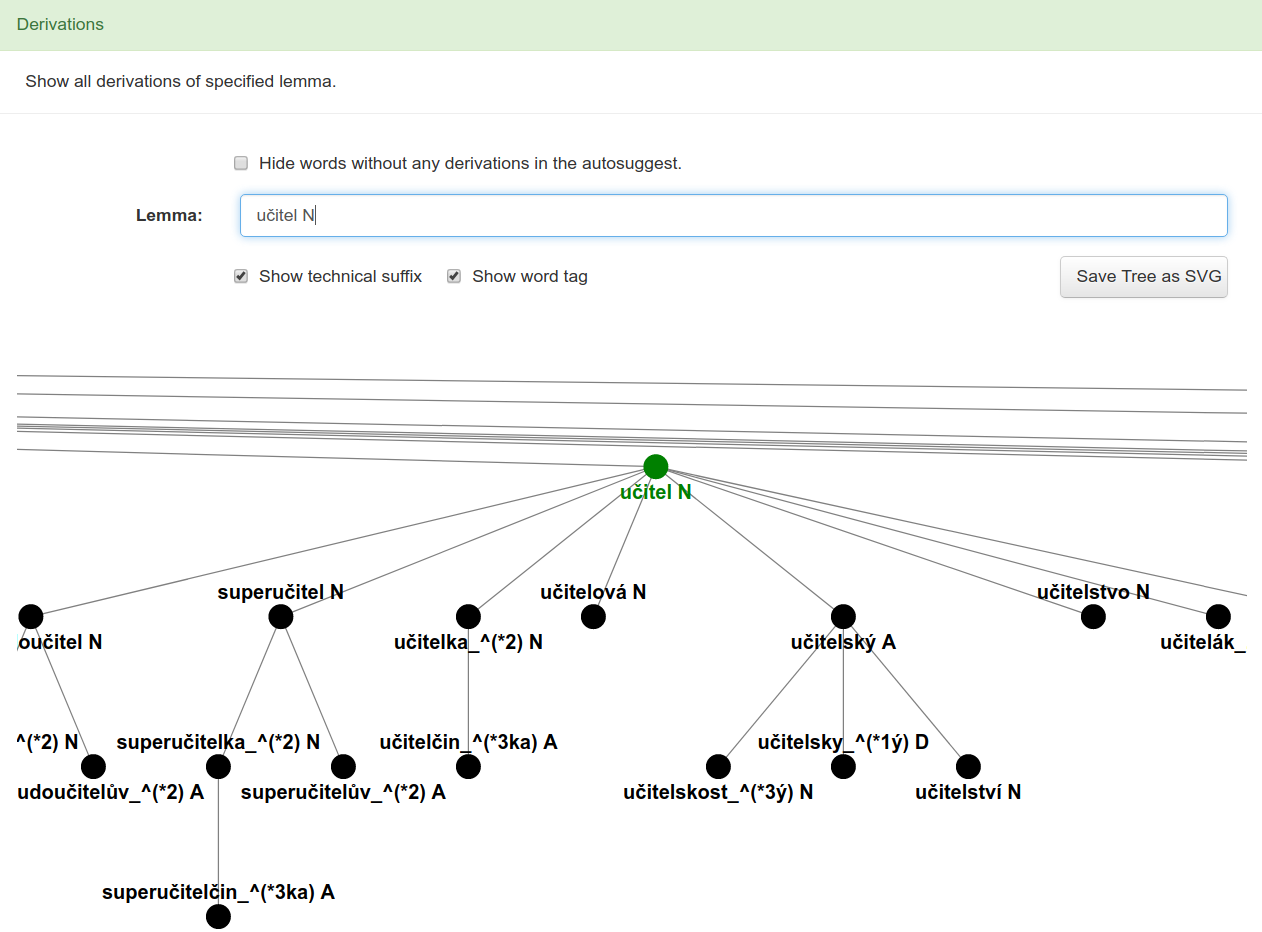
\includegraphics[width=.9\textwidth]{derinet-1}  
    \caption{Výsledný derivační strom v~prohlížeči DeriNet Viewer \parencite{derinet}}
    \label{derinet-1}
 \end{figure}

Aktuální verze derivační sítě DeriNet (1.7) obsahuje přibližně jeden
milion lemmat a~je dostupná skrze dvě webová uživatelská rozhraní.
Jedním z~nich je prohlížeč DeriNet
Viewer\footnote{Autor je Milan Straka -- http://ufal.mff.cuni.cz/derinet/derinet-viewer},
jehož základní funkcí je zobrazení derivačního stromu pro zadané lemma
(srov. obr. \ref{derinet-1}), případně lze vyhledané výsledky roztřídit
podle zvolených charakteristik. Druhý nástroj je DeriNet
Search\footnote{Autor je Jonáš Vidra -- http://ufal.mff.cuni.cz/derinet/search.},
který nabízí vyhledávání ve vlastním dotazovacím jazyce, to znamená, že
je uživatel schopen podle svých vlastních kritérii specifikovat omezení
pro tvar vyhledaného derivačního stromu. Například dotaz
\texttt{{[}pos="V"{]}\ ({[}pos="N"\ lemma="tel\$"{]},\ {[}pos="N"\ lemma="ce\$"{]})}
vyhledá takové derivační stromy, ve kterých je od verba přímo odvozeno
jednak substantivum končící sufixem \emph{-tel}, tak substantivum na
\emph{-ce} (viz obr. \ref{derinet-2}). \parencite{derinet-cz}

\begin{figure}[ht]   
    \centering
    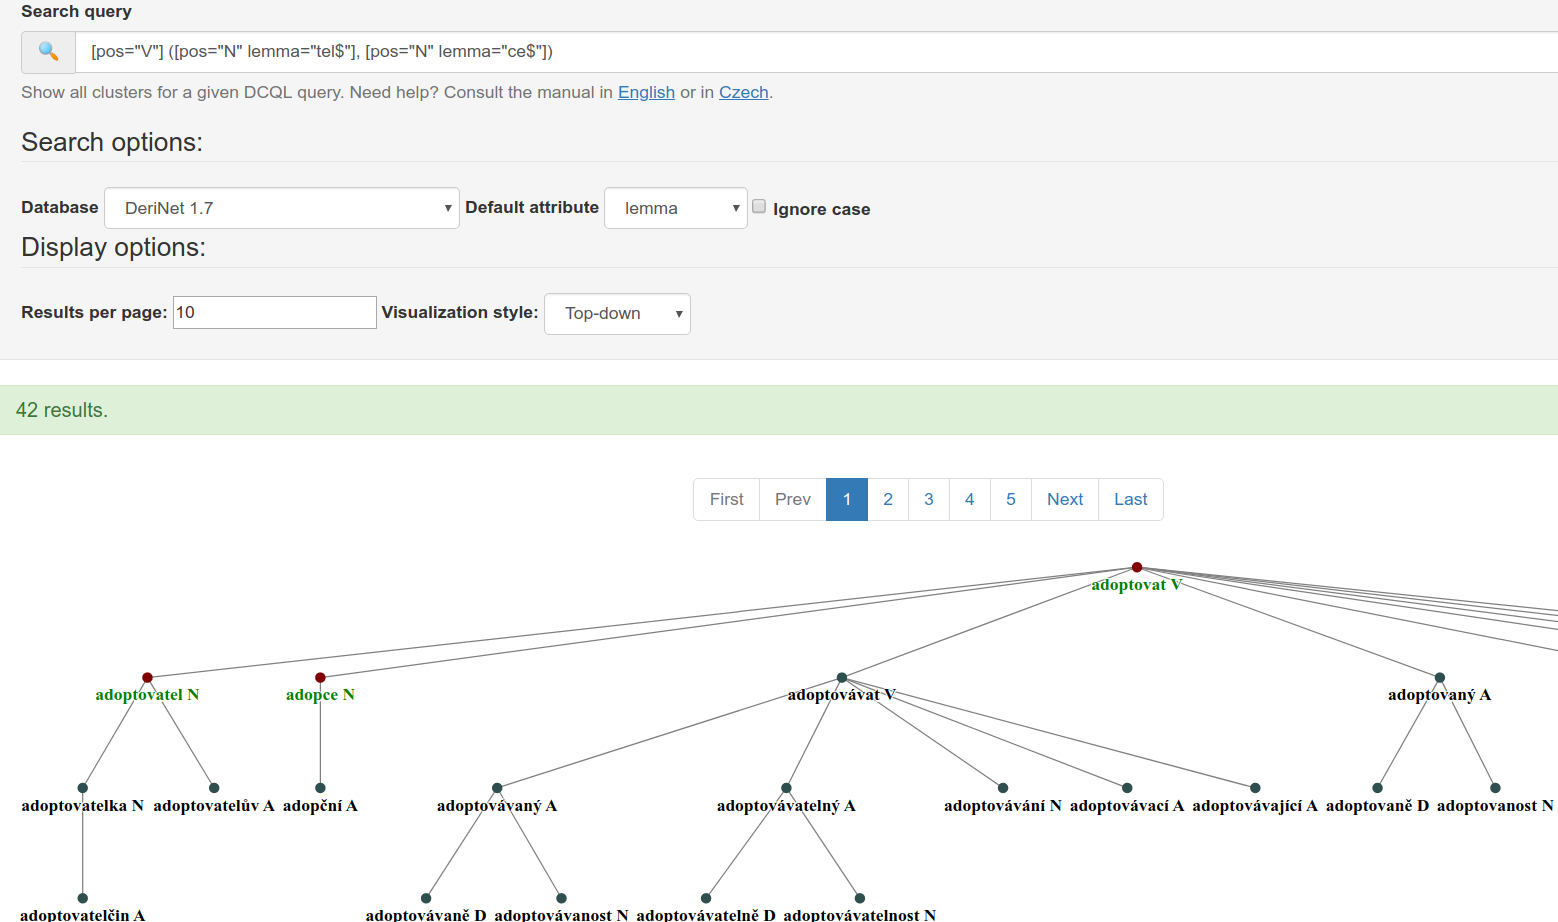
\includegraphics[width=.9\textwidth]{derinet-2}  
    \caption{Výsledek vyhledávacího dotazu ve vyhledávači DeriNet Search \parencite{derinet}}
    \label{derinet-2}
 \end{figure}

Další možnost, jak pracovat s~databází DeriNet, je prostřednictvím
jednoduchého datového formátu TSV (anglicky \emph{Tab-Separated Values}
-- jde o~textovou reprezentaci tabulkových dat, které jsou od sebe
odděleny tabulátorem), jenž je zpřístupněn k~volnému stažení pod licencí
Creative Commons Attribution-NonCommercial-ShareAlike 3.0 License.
U~tohoto přístupu se již počítá se základními programátorskými
dovednostmi, protože takto strukturovaná data primárně slouží jako vstup
pro určitý software. \parencite{derinet-cz}

\begin{verbatim}
692744  superuživatel   superuživatel   N   775428
775428  uživatel    uživatel    N   775440
775440  užívat  užívat_:T_^(*3t)    V   775402
775402  užít    užít_:T V   1006682
1006682 žít žít_:T  V
\end{verbatim}

Každý záznam (řádek) v~tomto souboru obsahuje několik atributů, jde
o~vlastní identifikační číslo, lemma, derivační informaci přejatou
z~morfologického slovníku MorFlex CZ, značku slovního druhu a~u~slov
derivovaných identifikační číslo slova základového -- tím je jednoznačně
vyznačen derivační vztah. Tento formát si můžeme ilustrovat na příkladu
derivačního řetězce \emph{žít} $\rightarrow$ \emph{užít}
$\rightarrow$ \ldots{} $\rightarrow$ \emph{superuživatel}. V~této
formě DeriNetu je reprezentován pěti záznamy, které jsou vzájemně
propojeny identifikačními čísly (poslední atribut odkazuje na první),
pouze u~značkového slovesa \emph{žít} žádný další odkaz neexistuje.
\parencite{derinet} A~právě tento formát DeriNetu slouží jako základ
derivačního slovníku v~rámci praktické části této práce.

\part{Praktická část}

\hypertarget{zpracovanuxe9-slovotvornuxe9-sufixy}{%
\chapter{Zpracované slovotvorné
sufixy}\label{zpracovanuxe9-slovotvornuxe9-sufixy}}

Cílem bakalářské práce bylo vytvořit elektronický slovník s~definicemi
založenými na derivačních rysech slovotvorně motivovaných slov ve formě
mobilní aplikace, proto si v~této kapitole praktické části popíšeme,
jaké slovotvorné sufixy byly zpracovány a~jakým způsobem probíhá proces
tvoření slovotvorných definic. V~druhé kapitole si pak rozebereme
technickou část spolu s~návrhem a~implementací samotné mobilní aplikace.

Při výběru slovotvorných typů ke zpracování byl brán zřetel na jejich
frekvenci a~produktivitu ve spojitosti s~derivací u~substantiv --
takovým nejvýraznějším typem jsou substantiva označující názvy živých
bytostí podle jejich činností zakončená na sufix \emph{-tel}, a~ta
spadají do slovotvorné třídy činitelských jmen.
\parencite[17]{dokulil67} V~této fázi je v~předkládané aplikaci
zpracován právě tento slovotvorný typ i~s~jeho rodovou alternativou
\emph{-telka}, jež má obdobné charakteristiky.

\hypertarget{slovotvornuxfd-typ--tel}{%
\section{Slovotvorný typ -tel}\label{slovotvornuxfd-typ--tel}}

\hypertarget{charakteristika}{%
\subsection{Charakteristika}\label{charakteristika}}

Pro účely této bylo důležité vybrat takový slovotvorný typ, u~něhož se
převážně shoduje slovotvorný a~lexikální význam. Tato podmínka je zde
splněna, protože z~1 129 zkoumaných lemmat zakončených sufixem
\emph{-tel} pouze u~3,03 \% z~nich strukturní význam neodpovídá významu
lexikálnímu (to se týká neživotných substantiv typu \emph{jmenovatel}
anebo takových substantiv, u~nichž je jejich slovesný základ sporný,
např. \emph{datel}) a~celkově je u~4,42 \% strukturní význam obecnější
(např.
\emph{vnímatel}\footnote{Význam slova vnímatel je dle SSJČ „kdo uvědoměle vnímá umělecké dílo“ \parencite{ssjc}, došlo tedy k~zúžení lexikálního významu.}).
Tento lingvistický výzkum byl založen na datech z~korpusu SYNv6
a~jednotlivé typy významů byly porovnávány prostřednictvím výkladových
slovníků. \parencite{adri}

Jak bylo již naznačeno, obecný význam činitelských jmen je podle
Dokulila definován jako „názvy osob a~živých bytostí vůbec podle povahy
a~druhu jejich činností`` \parencite[17]{dokulil67}. Sufix \emph{-tel}
tak vyjadřuje, že takto odvozený pojem je subjektem děje základového
slovesa s~tím, že nejčastěji jde
o~aktivní\footnote{To neplatí u~substantiv trpitel, truchlitel a~bydlitel, která jsou odvozena ze stavových sloves. \parencite[17]{dokulil67}}
účast subjektu na ději (např. subjekt označen slovem \emph{učitel}
vykonává takovou činnost, kterou vyjadřuje sloveso \emph{učit}, z~něhož
je výraz odvozený). U~tohoto slovotvorného typu se typicky jedná
o~mužská životná substantiva, nicméně se najdou i~výjimky v~podobě
neživotných substantiv (viz výše). \parencite{simandl2016}

Nejčastěji jsou substantiva tohoto slovotvorného typu odvozena od sloves
nedokonavých (imperfektiv), ze zkoumaných 1129 lemmat je jich takto
derivováno přibližně 74,3 \%, navíc se určitá část substantiv vzniklých
ze sloves dokonavých (perfektiv) chová tak, jako by byla odvozena
z~imperfektiv. Jde typicky o~názvy profesí (\emph{zastoupit}
$\rightarrow$ \emph{zastupitel}) a~názvy osob, pro které je daná
činnost typická, ale nejsou označovány za samostatné profese
(\emph{chovat} $\rightarrow$ \emph{chovatel}). Navíc je možné
sledovat progresivní tendenci produktivní V. slovesné třídy, v~níž
vznikají vedle tvarů utvořených z~perfektivních sloves
(\emph{zhotovitel}) i~tvary ze sloves imperfektivních
(\emph{zhotovovatel}). \parencite{adri}

\hypertarget{slovnuxedkovuxe9-heslo}{%
\subsection{Slovníkové heslo}\label{slovnuxedkovuxe9-heslo}}

Heslo derivačního slovníku se skládá ze tří částí:

\begin{itemize}
\tightlist
\item
  z~definice v~obecném slova smyslu;
\item
  derivační informace;
\item
  morfologické informace.
\end{itemize}

Definice je tvořena částečnou slovotvornou analýzou (segmentace slova na
slovotvornou bázi a~formant/y, například \emph{učitel} $\rightarrow$
\emph{učit-tel}) a~samotnou slovotvornou definicí založenou na
strukturním významu zadaného slova.

\hypertarget{slovotvornuxe1-definice}{%
\subsubsection{Slovotvorná definice}\label{slovotvornuxe1-definice}}

Slovotvorná definice je utvářena prostřednictvím dvou po sobě jdoucích
kroků -- v~prvním kroku dochází k~odhalení verbálního aspektu
fundujícího/motivující slovesa a~ve druhém se pak vstupnímu řetězci
přiřazuje jedna z~předem vytvořených definic.

\hypertarget{prvni-faze}{%
\subsubsection*{První fáze -- odhalení slovesného vidu}\label{prvni-faze}}

Verbální aspekt lze do určité míry vyextrahovat z~derivační sítě DeriNet
-- a~to analýzou slovotvorného řetězce:

\begin{itemize}
\tightlist
\item
  sloveso je perfektum: pokud řetězec obsahuje tutéž slovesnou formu
v~neprefigované podobě ve dvou předchozích slovotvorných krocích. Mějme
  například řetězec \emph{pracovat} (2. krok) $\rightarrow$
  \emph{\textbf{z}pracovat} (1. krok) $\rightarrow$
  \emph{zpracovatel} -- slovotvorná definice tak bude znít „ten, kdo
  zpracoval nebo zpracuje``;
\item
  sloveso je sekundární imperfektivum: pokud řetězec obsahuje rozdíl ve
  dvou předchozích slovotvorných krocích v~rámci specifického sufixu
u~jedné slovesné formy, příkladem může být řetězec \emph{pracovat}
  $\rightarrow$ \emph{zpracovat} (2. krok) $\rightarrow$
  \emph{zpraco\textbf{vá}vat} (1. krok) $\rightarrow$
  \emph{zpracovávatel} -- slovotvorná definice tak bude znít „ten, kdo
  zpracovává``;
\item
  sloveso je imperfektivum: pokud není perfektum a~zároveň není
  sekundární imperfektivum, například \emph{myslit} $\rightarrow$
  \emph{myslitel} -- slovotvorná definice je „ten, kdo myslí``.
\end{itemize}

\hypertarget{druha-faze}{%
\subsubsection*{Druhá fáze -- přiřazení definice}\label{druha-faze}}

Pro potřeby automatického zpracování jsme vytvářeli definice na základě
vlastních podvzorů, které jsou popsány určitými regulárními výrazy, viz
následující pravidla (dubletní varianty jsou označeny v~kulatých
závorkách):

\begin{itemize}
\tightlist
\item
  {[}\^{}ch{]}*ovatel\footnote{V tomto případě existují výjimky typu kl?ovatel, kdy zní definice u~neprefigovaného slovesa „ten, kdo kl?ove (kl?ová)“ a~u~prefigovaného „ten, kdo .*kl?oval nebo .*kl?ove (.*kl?ová). Mezi tato slova patří .*snovatel, .*plovatel, .*kovatel a~.*klovatel.}
  $\rightarrow$ Je prefigované?

  \begin{itemize}
  \tightlist
  \item
    ne $\rightarrow$ „ten, kdo .*uje``
  \item
    ano

    \begin{itemize}
    \tightlist
    \item
      Existuje ve slovotvorném řetězci sloveso ve tvaru .*ovat
      $\rightarrow$ „ten, kdo .*oval nebo .*uje``
    \item
      Existuje ve slovotvorném řetězci sloveso ve tvaru .*it nebo .*nout
      nebo .*{[}aá{]}t? $\rightarrow$ „ten, kdo .*uje``
    \end{itemize}
  \end{itemize}
\item
  .*chovatel $\rightarrow$ Je prefigované?

  \begin{itemize}
  \tightlist
  \item
    ne $\rightarrow$ „ten, kdo .*á``
  \item
    ano $\rightarrow$ „ten, kdo .*ten, kdo .*al nebo .*á``
  \end{itemize}
\item
  {[}\^{}o{]}*{[}iíyýaá{]}vatel $\rightarrow$ „ten, kdo
  .*{[}íýá{]}vá``
\item
  {[}\^{}o{]}*ěvatel $\rightarrow$ „ten, kdo .*ívá``
\item
  .*itel $\rightarrow$ Je prefigované?

  \begin{itemize}
  \tightlist
  \item
    ne

    \begin{itemize}
    \tightlist
    \item
      Je sloveso ve tvaru .*u.it? $\rightarrow$ „ten, kdo .*u.í``
    \item
      Je sloveso ve tvaru {[}\^{}u{]}*{[}eěi{]}t? $\rightarrow$ „ten,
      kdo .*í``
    \item
      Je sloveso ve tvaru .*u.ovat a~existuje zároveň ve slovotvorném
      řetězci sloveso ve tvaru .*ou.it? $\rightarrow$ „ten, kdo
      .*ou.il nebo .*ou.í``
    \end{itemize}
  \item
    ano

    \begin{itemize}
    \tightlist
    \item
      Existuje ve slovotvorném řetězci sloveso ve tvaru .*ou.it?
      $\rightarrow$ „ten, kdo .*ou.il nebo .*ou.í``
    \item
      Existuje ve slovotvorném řetězci sloveso ve tvaru .*ovat a~zároveň
      v~řetězci neexistuje sloveso ve tvaru .*it? $\rightarrow$ „ten,
      kdo .*oval``
    \item
      Je sloveso ve tvaru .*{[}eě{]}t? $\rightarrow$ „ten, kdo
      .*{[}eě{]}l nebo .*í``
    \item
      Je sloveso ve tvaru .*{[}\^{}ou{]}.*it $\rightarrow$ „ten, kdo
      .*il nebo .*í``
    \end{itemize}
  \end{itemize}
\item
  {[}\^{}zb{]}*atel\footnote{Zde do výjimek u~neprefigovaných podob spadají slova .*zobatel, .*hýbatel, .*kazatel a~.*tazatel.}
  $\rightarrow$ Je prefigované?

  \begin{itemize}
  \tightlist
  \item
    ne $\rightarrow$ „ten, kdo .*á``
  \item
    ano $\rightarrow$ „ten, kdo .*al nebo .*á``
  \end{itemize}
\item
  .*zatel $\rightarrow$ Je prefigované?

  \begin{itemize}
  \tightlist
  \item
    ne $\rightarrow$ „ten, kdo .*že``
  \item
    ano $\rightarrow$ ten, kdo .*zal nebo .*že``
  \end{itemize}
\item
  .*batel $\rightarrow$ Je prefigované?

  \begin{itemize}
  \tightlist
  \item
    ne $\rightarrow$ „ten, kdo .*bá`` (.*be)
  \item
    ano $\rightarrow$ „ten, kdo .*bal nebo .*bá`` (.*be)
  \end{itemize}
\item
  p{[}ií{]}satel $\rightarrow$ Je prefigované?

  \begin{itemize}
  \tightlist
  \item
    ne $\rightarrow$ „ten, kdo
    píše``\footnote{U nejfrekventovanějších slovesných tvarů, u~nichž v~rámci jednoho slovotvorného kroku docházelo k~výraznější hláskové alternaci, byla slovotvorná definice ručně specifikována -- jde například o~sloveso přemoci, jehož derivátem je činitelské jméno přemožitel.}
  \end{itemize}
\end{itemize}

Veškerá výše zmíněná pravidla jsou taktéž aplikovatelná na slovotvorný
typ \emph{-telka}, pro kterou je slovotvorná definice v~obecné rovině:
„ta, která .*``. Pokud budeme mít například za vstup slovo
\emph{vybudovatelka}, tak jeho definice bude znít „ta, která vybudovala
nebo vybuduje (vybudovat)``. Za definicí samotnou je v~závorce uvedeno
základové sloveso v~infinitivním tvaru, z~něhož bylo činitelské jméno
derivováno.

Slovník vytváří slovotvorné definice i~v~anglickém jazyce, v~rámci
kterého je definice zobecněná na „someone who .*`` s~tím, že je na konci
v~závorce specifikováno, o~jaký se jedná jedná rod. Příkladem může být
znovu výraz \emph{vybudovatelka} s~anglickou definicí „someone who
builds (feminine)``.

\hypertarget{derivaux10dnuxed-a-morfologickuxe1-informace}{%
\subsubsection{Derivační a~morfologická
informace}\label{derivaux10dnuxed-a-morfologickuxe1-informace}}

Kromě hlavní definice slovníkové heslo obsahuje ještě dodatečnou
derivační a~morfologickou informaci. První z~nich obsahuje základové
slovo, z~něhož byl vstupní výraz odvozen, a~typ derivačního procesu --
v~případě tohoto slovotvorného typu se jedná o~sufixaci.

Morfologická informace se pak skládá ze slovního druhu vstupního výrazu,
z~jeho rodu a~z~určitého morfologického paradigmatu, do něhož bylo slovo
zařazeno.

\hypertarget{elektronickuxfd-derivaux10dnuxed-slovnuxedk}{%
\chapter{Elektronický derivační
slovník}\label{elektronickuxfd-derivaux10dnuxed-slovnuxedk}}

V~této kapitole popisujeme výsledek praktické části, a~to jak z~hlediska
formálních požadavků na nástroj jako takový, tak z~hlediska procesu
návrhu a~implementace.

Derivační slovník je primárně koncipován jako edukační pomůcka pro
cizince, kteří se učí češtinu jako druhý jazyk. Na rozdíl od rodilých
mluvčí nedokážou cizinci podvědomě predikovat význam neznámých slov na
základě slovotvorných morfému v~určitých kontextech. Chybí jim tedy
podvědomá znalost významů určitých slovotvorných afixů, prostřednictvím
kterých by si pak dokázali analogicky vyvodit význam slova neznámého.

Věříme, že by se tento slovník mohl stát dobrou učební pomůckou, pomocí
které by mohli cizinci porozumět např. takovým internacionalismům, které
byly přejaty do slovotvorného systému českého jazyka pomocí sufixů.

Díky pravidelnému využívání slovníku taktéž očekáváme zejména u~cizinců
se slovanským rodným jazykem (z~důvodu flektivního charakteru těchto
jazyků) rychlejší akvizici derivačních vztahů a~principů v~češtině.

\hypertarget{poux17eadavky-na-aplikaci}{%
\section{Požadavky na aplikaci}\label{poux17eadavky-na-aplikaci}}

Cílem práce bylo vytvořit derivační slovník ve formě mobilní aplikace,
který bude využívat slovotvorných informací z~derivační sítě DeriNet.
Dílčím požadavkem, který vychází přímo z~povahy samotného slovníku
jakožto podpůrného nástroje pro výuku cizinců, bylo vyhledat
a~implementovat dvojjazyčný česko-anglický slovník, a~to proto, aby byla
celá aplikace včetně slovotvorných definic kompletně lokalizovaná
v~anglickém jazyce.

Požadavky na funkcionalitu slovníku jako takového můžeme ve stručnosti
shrnout v~následujících bodech:

\begin{itemize}
\tightlist
\item
  funkce \emph{insert word} $\rightarrow$ vrátí se zadaného vstupu:

  \begin{itemize}
  \tightlist
  \item
    částečnou slovotvornou analýzu;
  \item
    anglickou i~českou definici založenou na strukturním významu slova
    (anglickou pouze v~případě, že se takový ekvivalent bude nacházet ve
    vybraném česko-anglickém slovníku);
  \item
    doplňující derivační a~morfologické informace;
  \end{itemize}
\item
  heslář již zpracovaných slov ve formě rejstříku.
\end{itemize}

Součástí zadání také bylo to, aby všechny funkcionality mobilní aplikace
byly kompletně funkční bez připojení k~internetu -- tím pádem nebylo
zapotřebí řešit autentifikaci
uživatele\footnote{Nicméně je tato možnost stále v~řešení, a~to pro případ, kdybychom v~aplikaci chtěli nabídnout možnost ukládání již naučených hesel do osobního adresáře atd.}
či pracovat se vzdáleným uložištěm.

\hypertarget{nuxe1vrh-aplikace}{%
\section{Návrh aplikace}\label{nuxe1vrh-aplikace}}

Na začátku samotného vývoje si je zapotřebí určit několik věci, v~našem
případě jde primárně o:

\begin{itemize}
\tightlist
\item
  zvolení vhodných technologií včetně programovacího jazyka, kterými
  budeme nástroj implementovat;
\item
  návrh uživatelského rozhraní aplikace spolu s~navigací mezi
  jednotlivými vizuálními prvky (včetně konkrétních přechodů).
\end{itemize}

\hypertarget{pouux17eituxe9-technologie}{%
\subsection{Použité technologie}\label{pouux17eituxe9-technologie}}

Tradiční způsob vývoje mobilních aplikací se obecně dělí na tři hlavní
typy -- jde o~takzvané webové, nativní a~hybridní aplikace. Každý
z~těchto přístupů má svá vlastní pozitiva a~negativa, a~tedy si je
zapotřebí na začátku každého vývoje určit, pro jaké účely má daná
aplikace sloužit a~jaké funkcionality splňovat.

Webové aplikace fungují typicky na všech platformách a~jsou založeny na
klasických webových technologiích, tzn. na HTML, CSS a~na programovacím
jazyce JavaScript (viz podkapitola \ref{webovuxe9-technologie}), jedná
se tedy o~přizpůsobené webové stránky, z~čehož vyplývá potřeba
internetového připojení. Výhodou tohoto přístupu je kromě již zmíněné
multiplatformní povahy ukládání dat na webových serverech, tyto aplikace
tak nevyžadují velké množství paměti na lokálním uložišti. Za hlavní
negativum je považována nižší kompatibilita s~hardwarem a~operačním
systémem u~daných mobilních zařízení.

Na druhou stranu nativní aplikace jsou vyvíjeny pouze pro jednu
specifickou platformu, to znamená, že například aplikaci vytvořenou pro
systém Android nelze spustit na systému iOS a~naopak. Z~tohoto přístupu
vyplývají výhody ve formě maximálního využití daného operačního systému
(větší výkon, kompatibilita, uživatelská zkušenosti, \ldots), ale
i~nevýhody týkající se nutnosti využívání specifických technologií
určitého operačního systému (například pro operační systém iOS se
využívá programovací jazyk Objective-C (nově Swift), pro Android je
určen jazyk Java).

Posledním typem jsou pak hybridní aplikace, které kombinují oba předešlé
přístupy -- vývoj probíhá ve specializovaném nástroji za použití
webových technologií, v~rámci kterého se testuje logika jednotlivých
funkcionalit. Po jeho dokončení dochází ke kompilaci do vybraného
operačního systému, v~rámci kterého se již pracuje s~klasickými
nativními funkcemi (například s~mikrofonem, fotoaparátem, lokálním
uložištěm v~telefonu atd.). Výhoda hybridních aplikací je
v~jednoduchosti vývoje, který je v~porovnání s~nativním rychlý a~snadný,
a~to i~z~toho důvodu, že se u~něj pracuje pouze s~jedním zdrojem kódu,
který je však použitelný na větší počet platforem. Negativním aspektem
je pak pomalejší výpočetní výkon, který je spojen s~využitím speciálních
knihoven pro převod do výsledné podoby mobilní aplikace.

Jelikož se v~našem případě pracuje s~minimem nativních funkcí, aplikace
by měla být nezávislá na internetovém připojení a~jde nám spíše
o~rozšíření nástroje napříč různými platformami, zvolíme hybridní formu
vývoje.

\hypertarget{webovuxe9-technologie}{%
\subsubsection{Webové technologie}\label{webovuxe9-technologie}}

Jak bylo výše poznamenáno, vývoj hybridních aplikací probíhá
prostřednictvím klasických webových technologií, do nichž spadá HTML,
CSS a~JavaScript, proto si je v~následujících odstavcích v~krátkosti
popíšeme.

HTML (Hypertext Markup Language) a~CSS (Cascading Style Sheets) jsou dvě
základní technologie, na nichž jsou v~nejobecnější rovině postaveny
webové stránky. HTML je značkovací jazyk, pomocí kterého popisujeme
strukturu webových stránek, což znamená, že za použití speciálně
definovaných značek přiřazujeme jednotlivé významy částem obsahu. Pomocí
CSS pak nastavujeme vizuální podobu dané webové stránky (barvy, fonty,
odsazení atd.). Důležitou vlastností CSS je nezávislost na HTML, můžeme
tedy dle potřeby tyto dva jazyky separovat a~následně s~mírnými obměnami
využít v~rámci jiného projektu/prostředí. \parencite{htmlcss}

Před samotným vykreslením určité webové stránky musí dojít k~převedení
HTML dokumentu do objektu zvaného DOM (Document Object Model) -- jde
o~HTML uložené ve stromové struktuře, kde je o~každém jednotlivém uzlu
(tedy značce) uložená informace o~jeho lokaci. S~tímto objektem dále
pracuje CSS (aplikují se jednotlivá pravidla týkající se vykreslení)
a~JavaScript, jehož prostřednictvím se pak může dynamicky měnit struktura
a~zobrazení tohoto stromového objektu. \parencite{howbrowserswork}

JavaScript (obecněji ECMAscript) je
skriptovací\footnote{Jako skriptovací jazyk je označován z~toho důvodu, že není při svém spuštění nijak kompilován (například na rozdíl od programovacích jazyků jako jsou Java nebo Objective-C) a~namísto toho je rovnou proveden daným webovým prohlížečem (ten je tak jeho interpretem).}
programovací jazyk, který je součástí všech moderních webových
prohlížečů. JavaScript se používá na takových místech, kde je zapotřebí
v~rámci webové stránky určitým způsobem interagovat s~jejím uživatelem,
to znamená, že ho typicky využijeme v~oblasti webových aplikací, u~nichž
je očekávaný zásah uživatele a~je zapotřebí dynamicky měnit zobrazovaný
obsah. \parencite{javascript}

\hypertarget{framework-ionic-a-angular}{%
\subsubsection{Framework Ionic a~Angular}\label{framework-ionic-a-angular}}

Při vývoji komplexnějších webových a~mobilních aplikací se často pracuje
s~takzvanými webovými frameworky, které určitým způsobem zjednodušují
vývoj. Ve stručnosti je jejich účelem umožnit vývojářům práci v~takovém
prostředí, v~němž se mohou primárně zaměřit na požadavky daného projektu
a~nemusí řešit problematiku opakujících se funkcí nebo závislosti
jednotlivých knihoven.

My jsme v~rámci naší mobilní aplikace využili Ionic Framework, což je
soubor nástrojů s~otevřeným zdrojovým kódem pod licencí
MIT\footnote{https://opensource.org/licenses/MIT}, který se zaměřuje na
uživatelské rozhraní u~mobilních a~webových aplikací. Obsahuje velké
množství vizuálních komponent, jež jsou typické pro mobilní zařízení,
a~taktéž je zde umožněno pomocí knihovny Ionic Native přistupovat
k~nativním funkcím mobilního zařízení -- zde se využívá knihovna Cordova,
která slouží pro převod webové aplikace do aplikace mobilní.
\parencite{cordova}

Dalším cílem Ionicu je poskytnout takové prostředí pro vývoj hybridních
aplikací, které je kompatibilní s~dalšími frameworky, jako jsou
například React nebo Vue, nicméně jeho jádro a~struktura samotného kódu
je založena na webovém frameworku Angular. \parencite{ionic}

Angular jako takový pracuje s~programovacím jazykem TypeScript, který je
vyvíjen firmou Microsoft jako open-source. TypeScript je rozšíření již
zmíněného JavaScriptu, to v~praxi znamená, že kód napsaný v~TypeScriptu
je zapotřebí nejdříve převést do určité podoby javaScriptového standardu
a~ten je až poté možné interpretovat ve webových prohlížečích. Tento
programovací jazyk se používá primárně z~důvodu své silné typové
kontroly. Pokud je tedy této možnosti využito, lze tak díky ní
předcházet mnohým potenciálním chybám. \parencite{typescript}

Architektura frameworku Angular se skládá z~mnoha vzájemně provázaných
vrstev, ve stručnosti popíšeme právě ty, které jsou pro pochopení naši
aplikace klíčové. Základním prvkem architektury jsou \emph{komponenty},
v~rámci kterých dochází k~propojení aplikační logiky s~konkrétní HTML
šablonou a~CSS (ty společně určují celkový vzhled). Jedna komponenta je
většinou rovna jedné vizuální stránce v~aplikaci, nicméně Angular dokáže
svými vlastními značkami (\emph{direktivami}) ovlivnit výslednou podobou
šablony ještě před jejím zobrazením -- díky tomuto principu jednoduše
dochází k~dynamické proměně obsahu stránek podle zadané aplikační
logiky, protože ta ovlivňuje chování samotných direktiv. Další důležitou
části jsou \emph{služby} -- ty už nejsou propojeny s~žádnou vizuální
stránkou (s~HTML šablonou), ale slouží pro dekompozici jednotlivých
funkcionalit napříč aplikací. Data, která jsou těmito službami
zpracována, jsou pak dále přeposílána do určitých komponent.
\parencite{angulararchitecture}

\hypertarget{nuxe1vrh-uux17eivatelskuxe9ho-rozhranuxed}{%
\subsection{Návrh uživatelského
rozhraní}\label{nuxe1vrh-uux17eivatelskuxe9ho-rozhranuxed}}

V~této podkapitole popíšeme hlavní vizuální prvky uživatelského rozhraní
a~zaměříme se zde na popis chování rozhraní při interakci s~uživatelem.
Návrh celého uživatelského rozhraní přímo vychází z~požadavků na
aplikaci jako takovou (viz \ref{poux17eadavky-na-aplikaci}) a~je
demonstrován na mobilním telefonu s~operačním systémem Android.

První obrazovka, se kterou uživatel přichází do styku po spuštění
aplikace, je úvodní stránka, která uvádí základní informace o~derivačním
slovníku (viz obrázek \ref{1}). Pod těmito informacemi se vyskytují dvě
velká navigační tlačítka (\emph{open index} a~\emph{search}), která
uživatele vedou k~využití hlavních funkcionalit aplikace.

\begin{figure}[ht]
  \begin{subfigure}[b]{0.45\textwidth}
    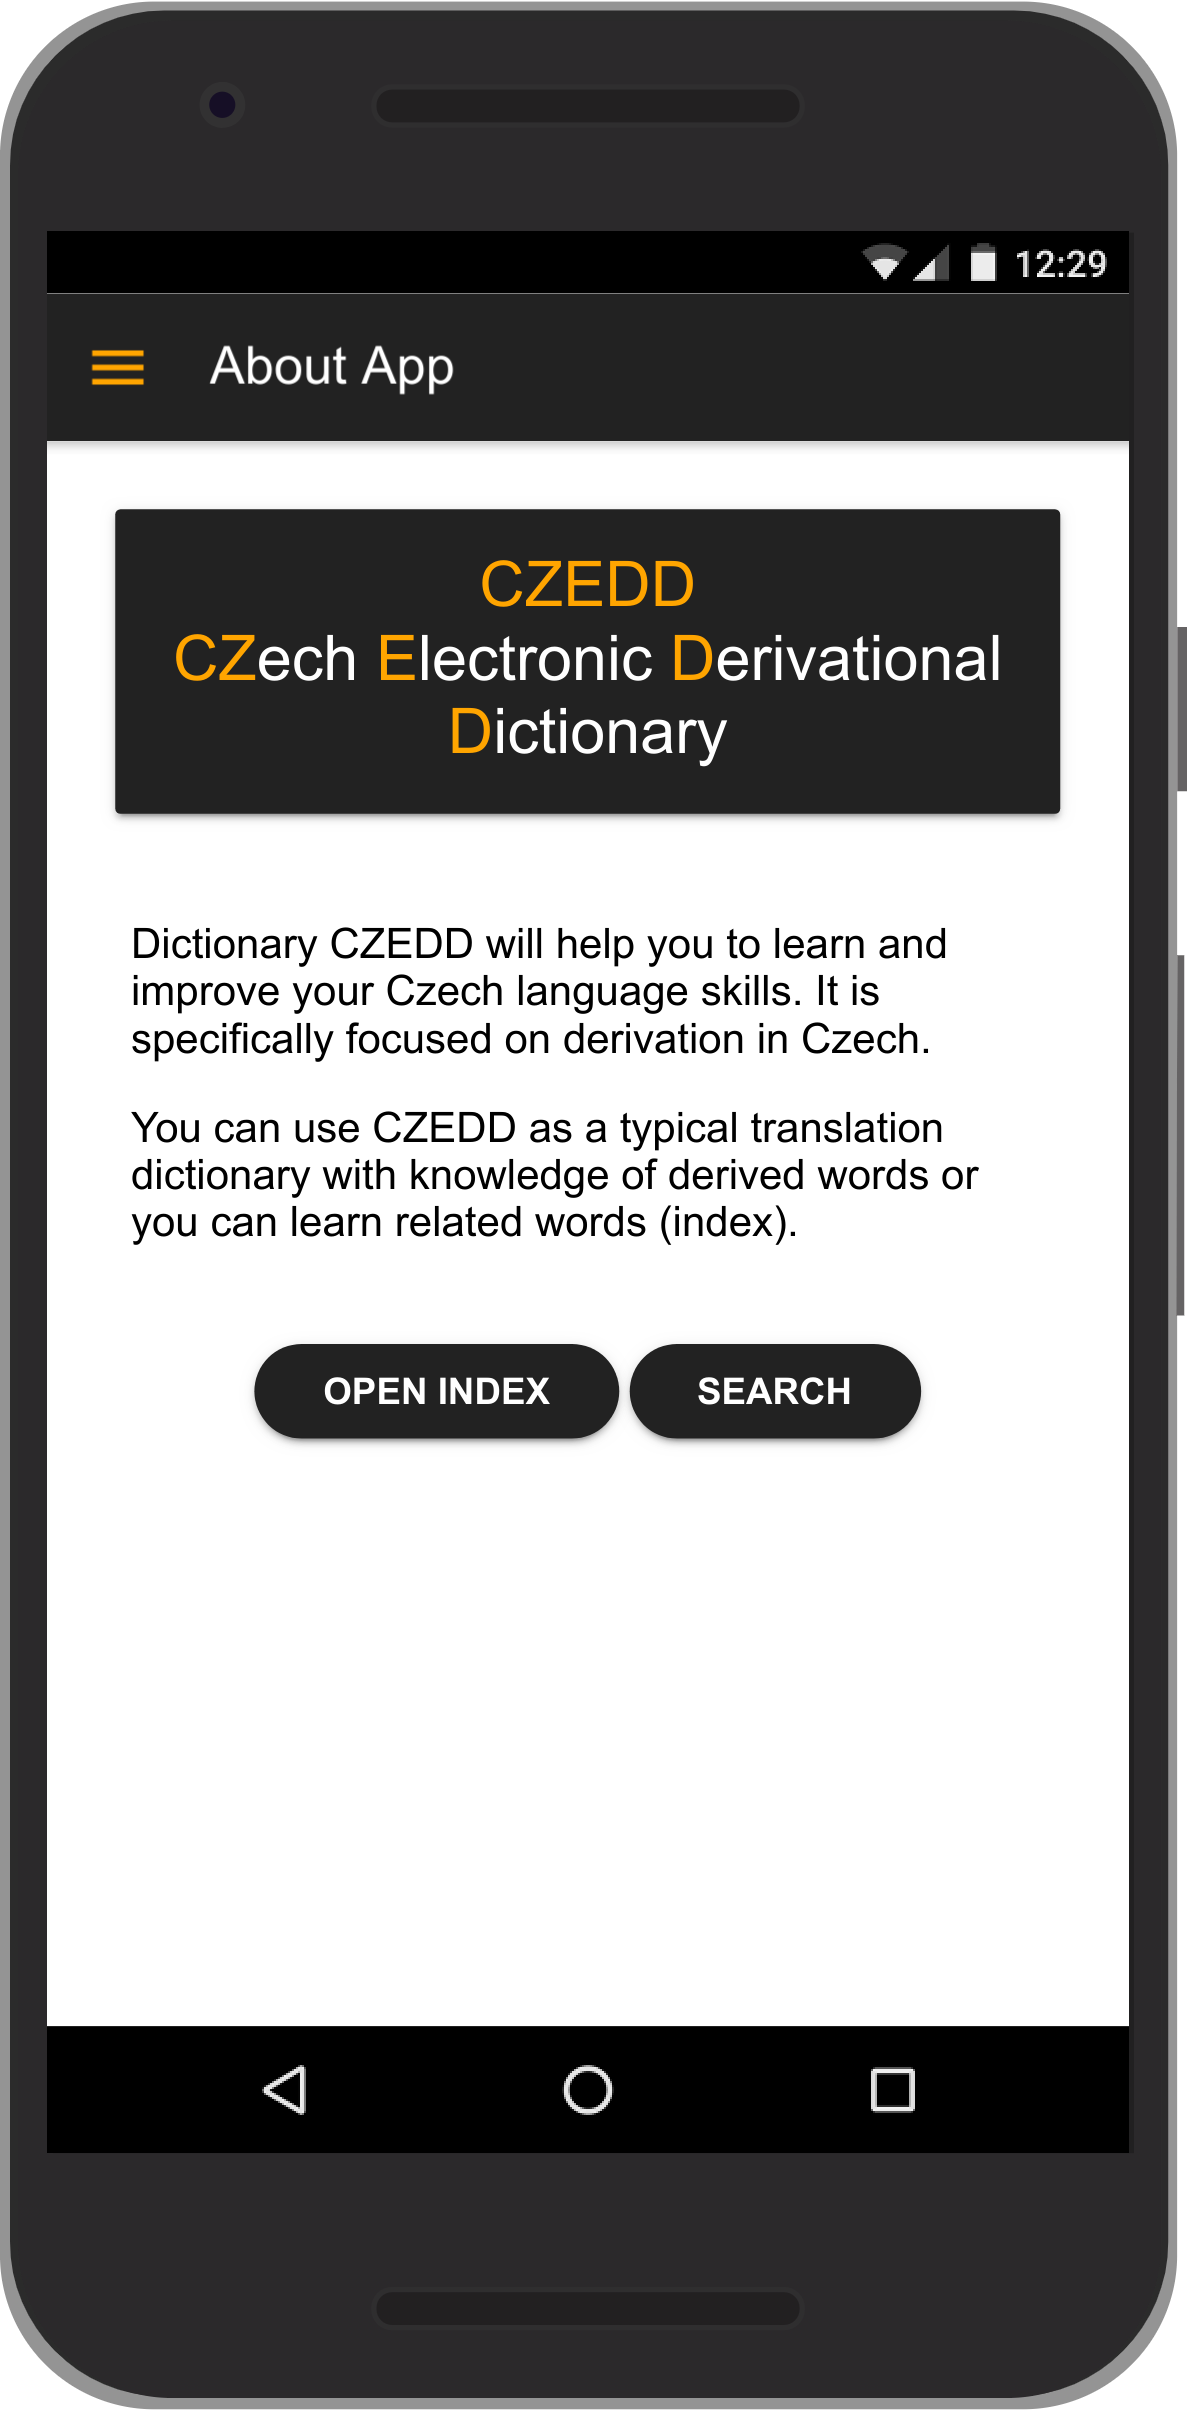
\includegraphics[width=0.9\textwidth]{1-1}
  \end{subfigure}
  \hfill
  \begin{subfigure}[b]{0.45\textwidth}
    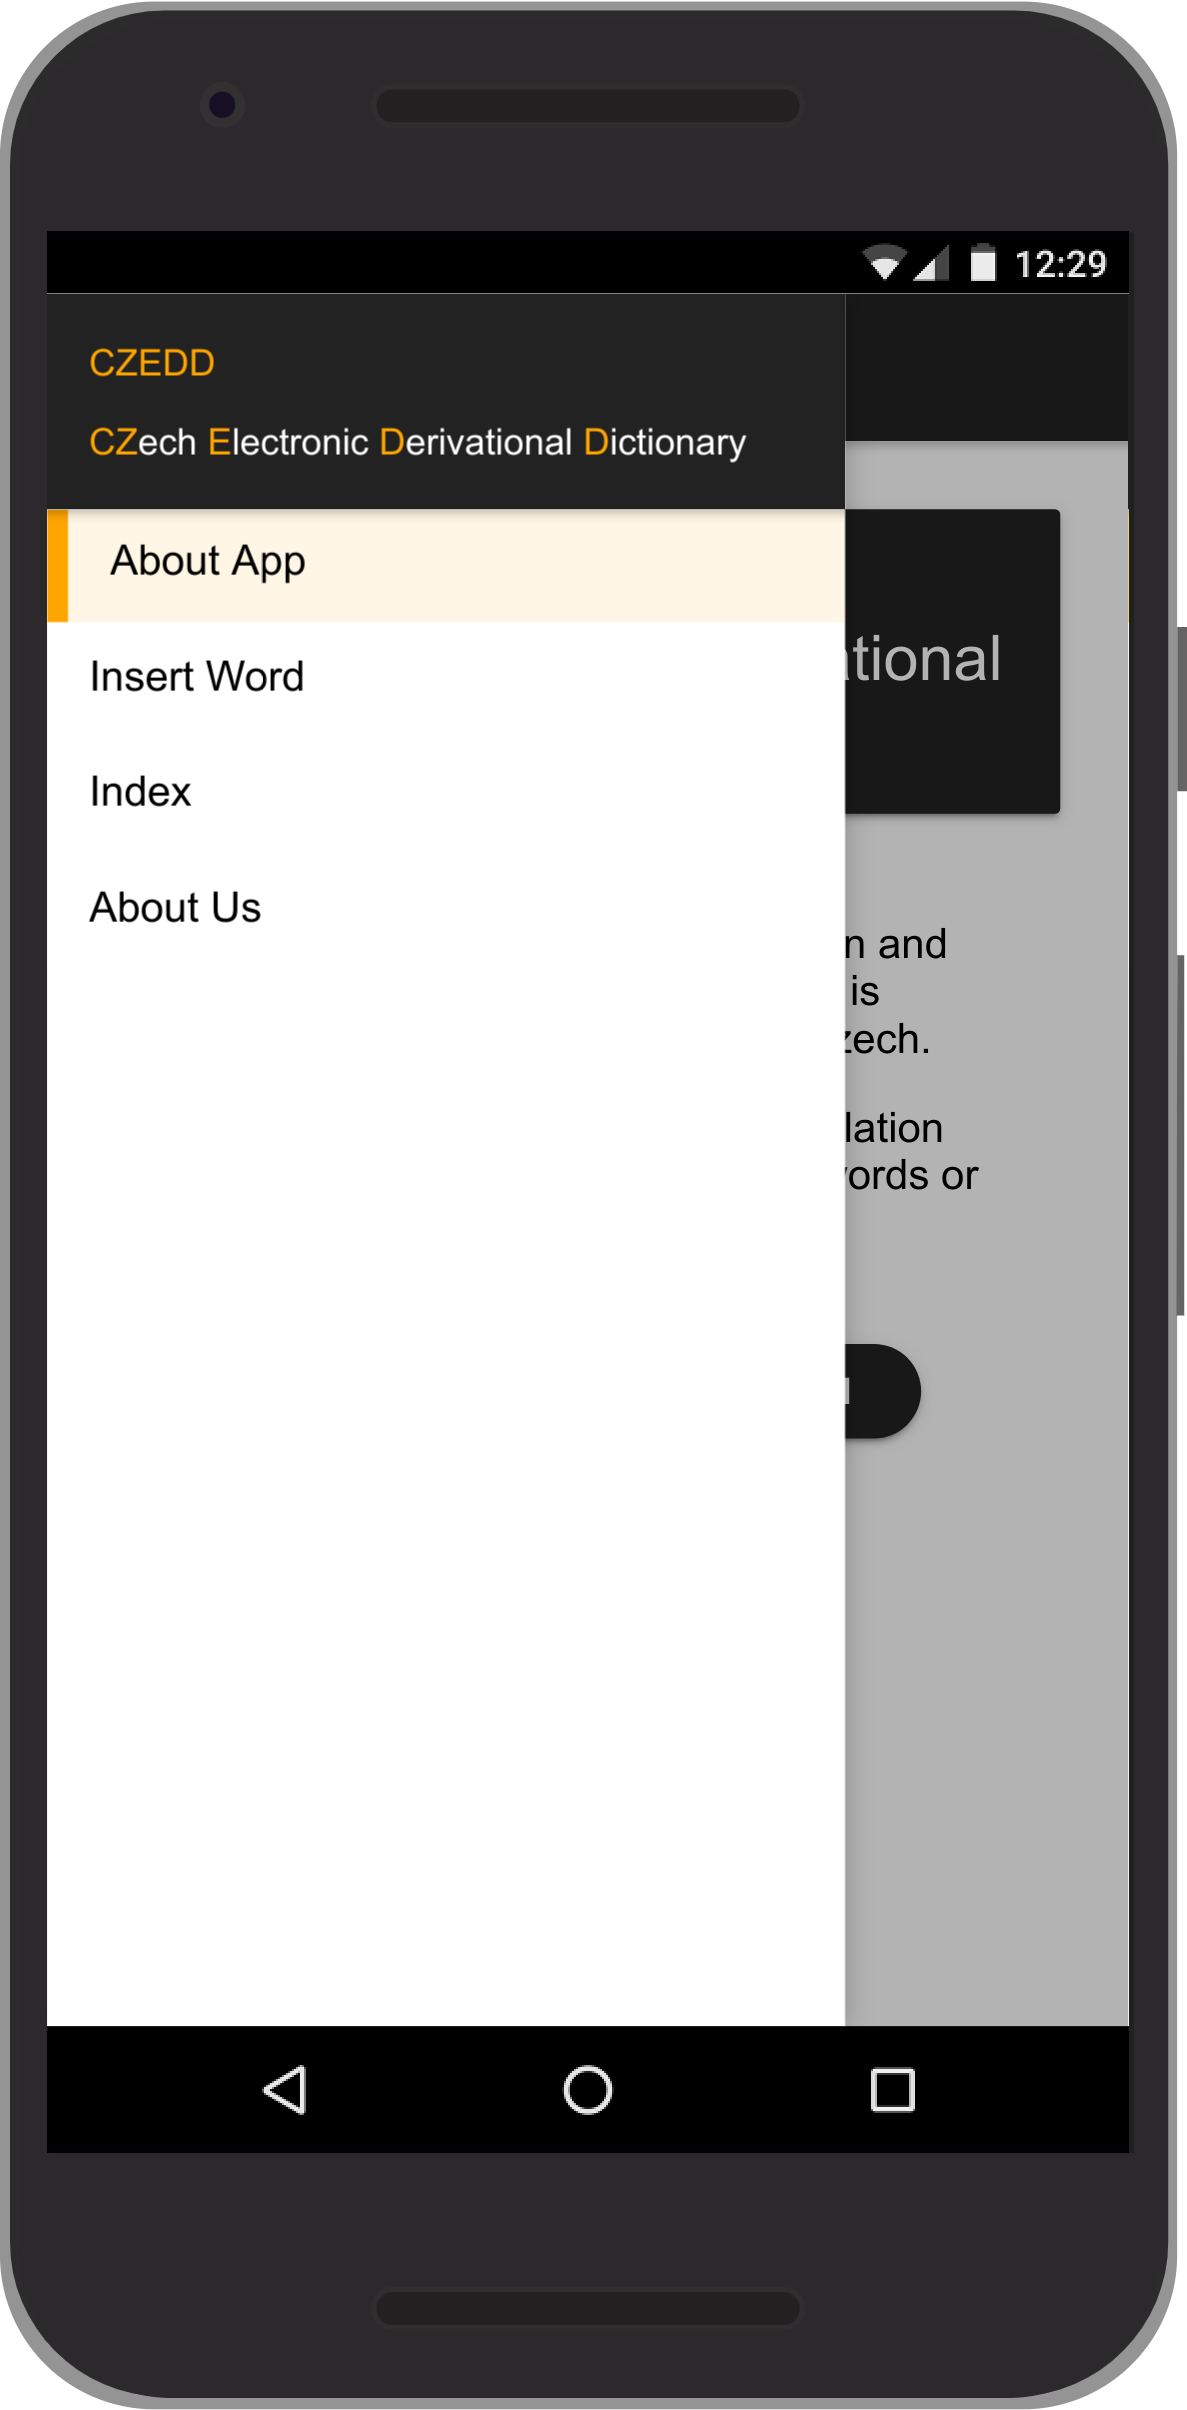
\includegraphics[width=0.9\textwidth]{1-2}
  \end{subfigure}
  \caption{Úvodní stránka a~navigační menu}
  \label{1}
\end{figure}

Druhá možnost, jak využít navigačního systému aplikace, je pomocí
navigačního vysouvacího menu (viz obrázek \ref{1}), jež nabízí čtyři
možná přesměrování. Barevnou indikací je vždy označena aktuální pozice
uživatele v~systému -- tohle menu je vždy přístupné v~levém horním rohu
obrazovky.

Nejdůležitějším prvkem celého uživatelského rozhraní je přístup k~hlavní
funkcionalitě \emph{insert word}. Domníváme se, že právě zde musí dojít
k~co nejpříjemnějšímu uživatelskému zážitku, protože na tomto místě
dochází k~uspokojení, či neuspokojení potřeb uživatele vzhledem
k~aplikaci.

S~ohledem na výše zmíněné je výchozím stavem prázdné textové pole, které
očekává vstup od uživatele. Po zadání jednotlivých znaků obrazovka
dynamicky zobrazuje pouze ta slova z~rejstříku zpracovaných slov, která
začínají podřetězcem zadaného slovního tvaru (viz obrázek \ref{2}).
A~právě přes tato vyselektovaná slova se lze dostat k~výslednému
slovníkovému heslu.

\begin{figure}[ht]
  \begin{subfigure}[b]{0.3\textwidth}
    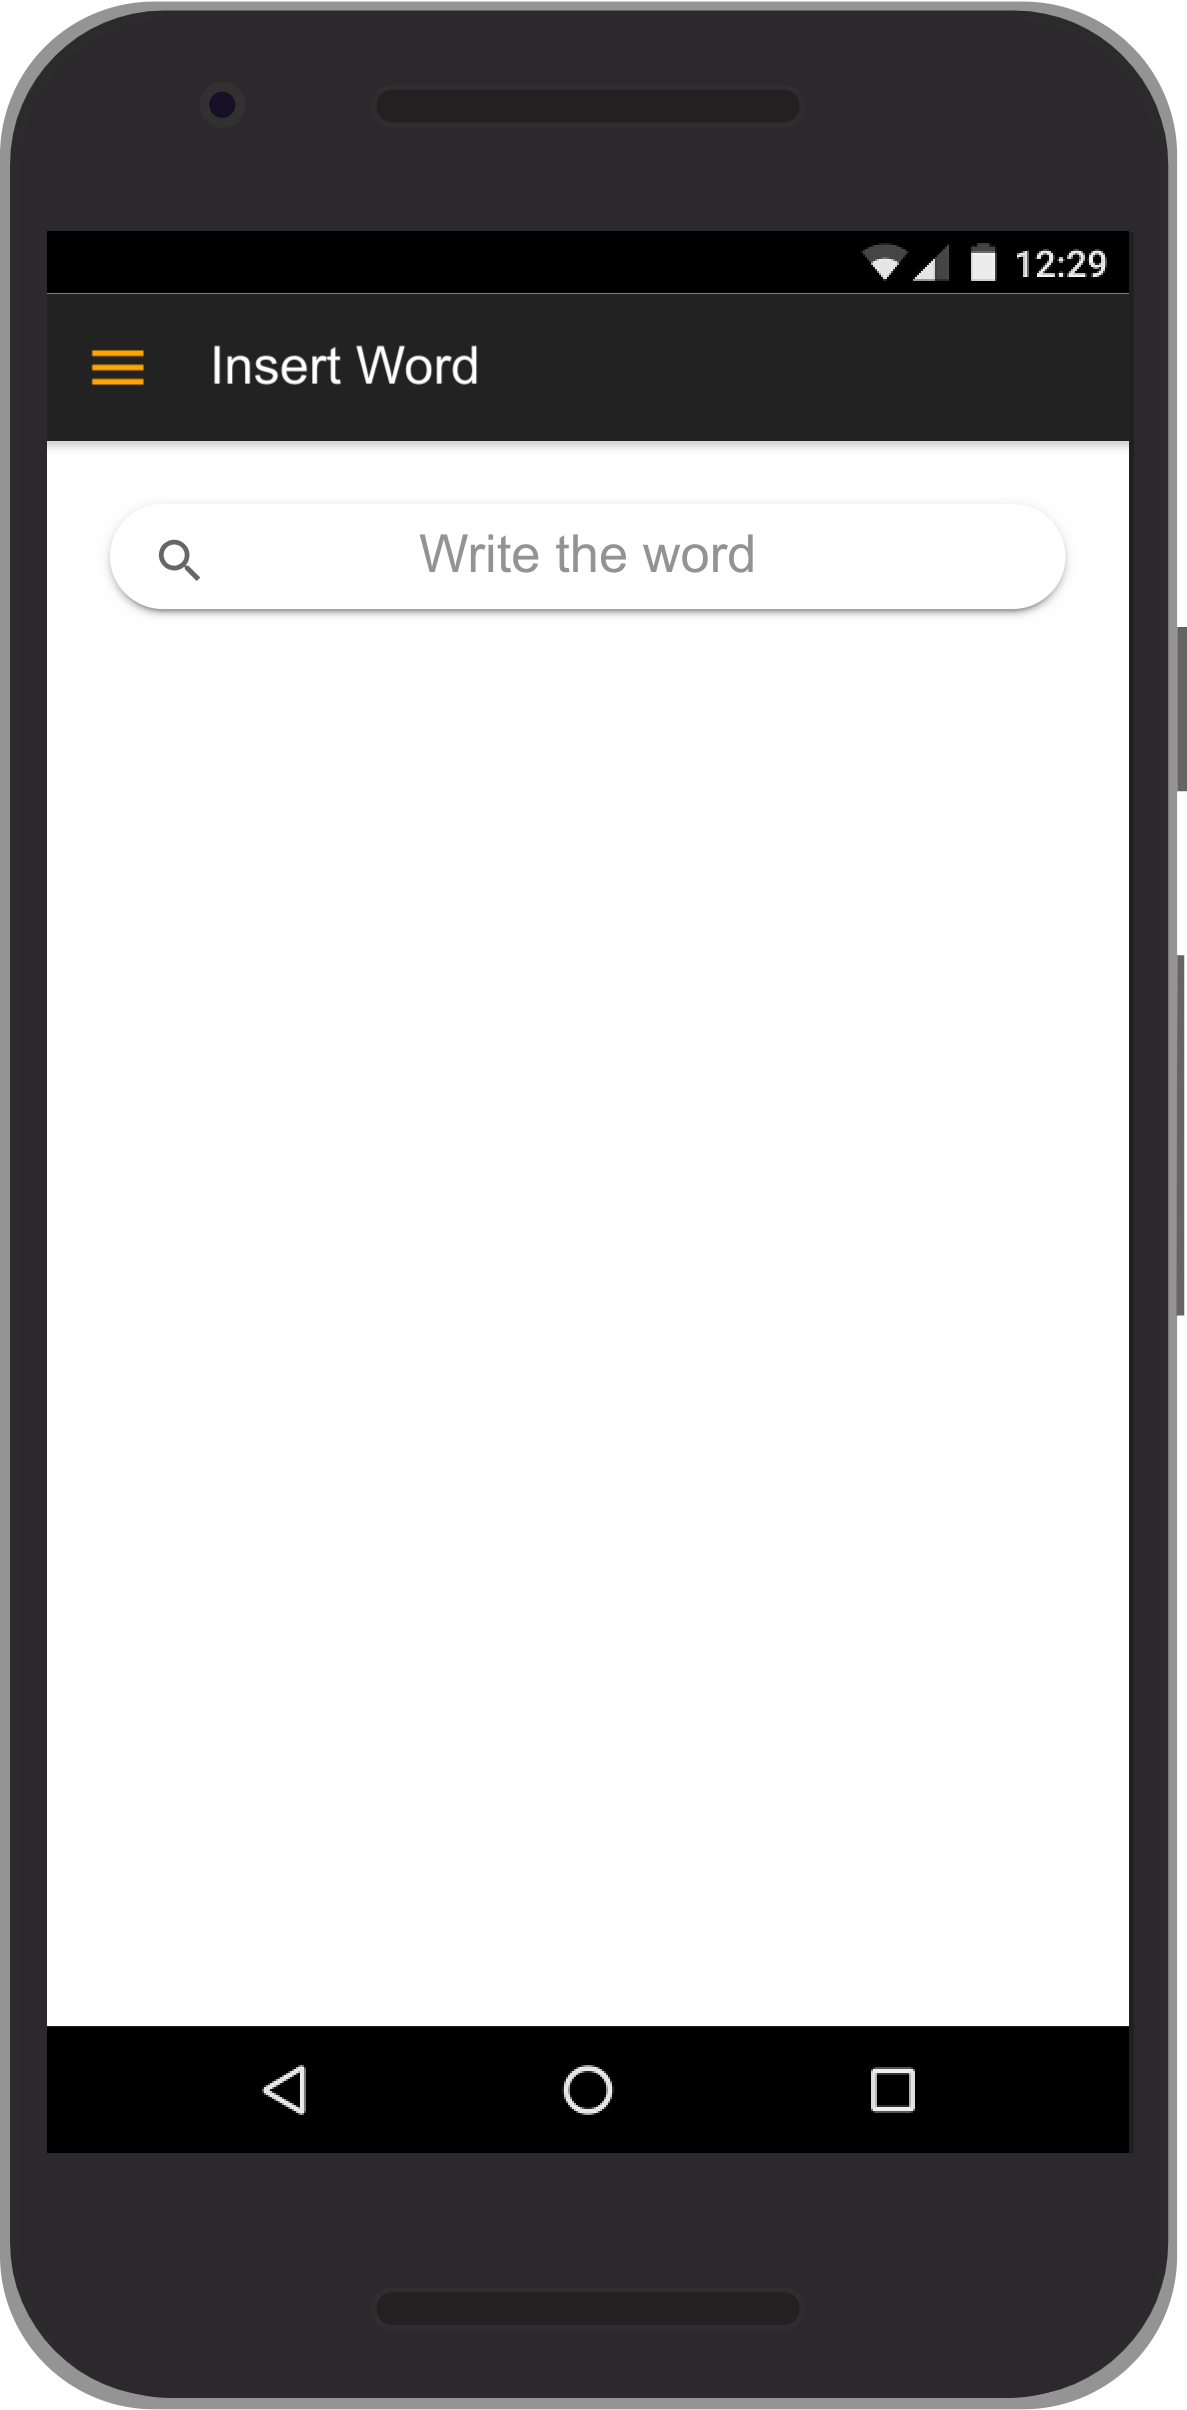
\includegraphics[width=\textwidth]{2-1}
  \end{subfigure}
  \hfill
  \begin{subfigure}[b]{0.3\textwidth}
    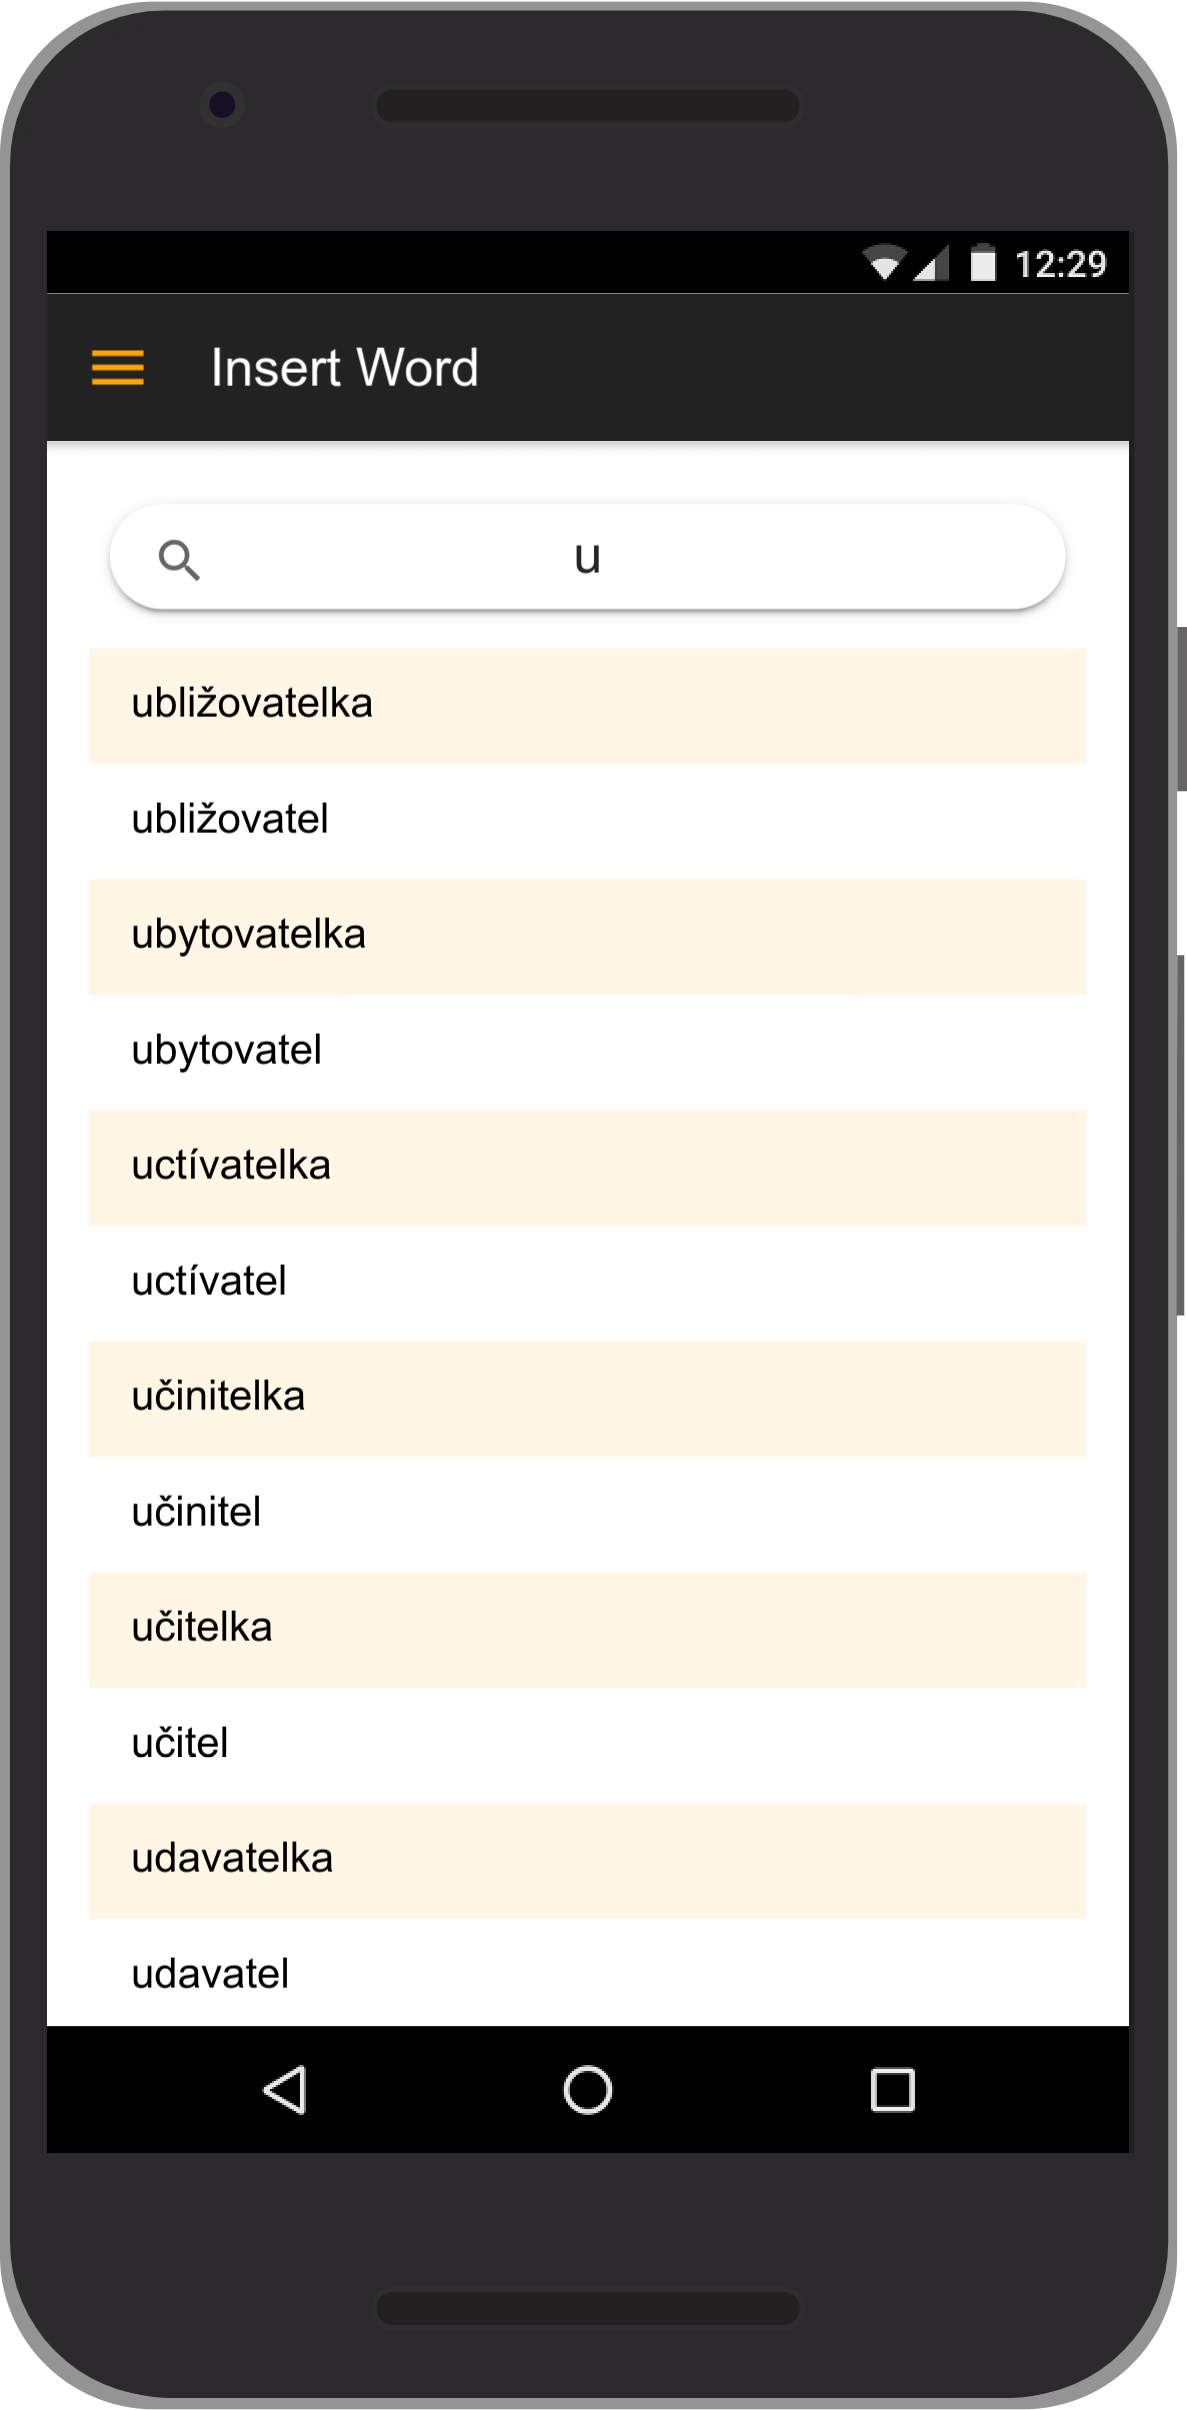
\includegraphics[width=\textwidth]{2-2}
  \end{subfigure}
   \hfill
  \begin{subfigure}[b]{0.3\textwidth}
   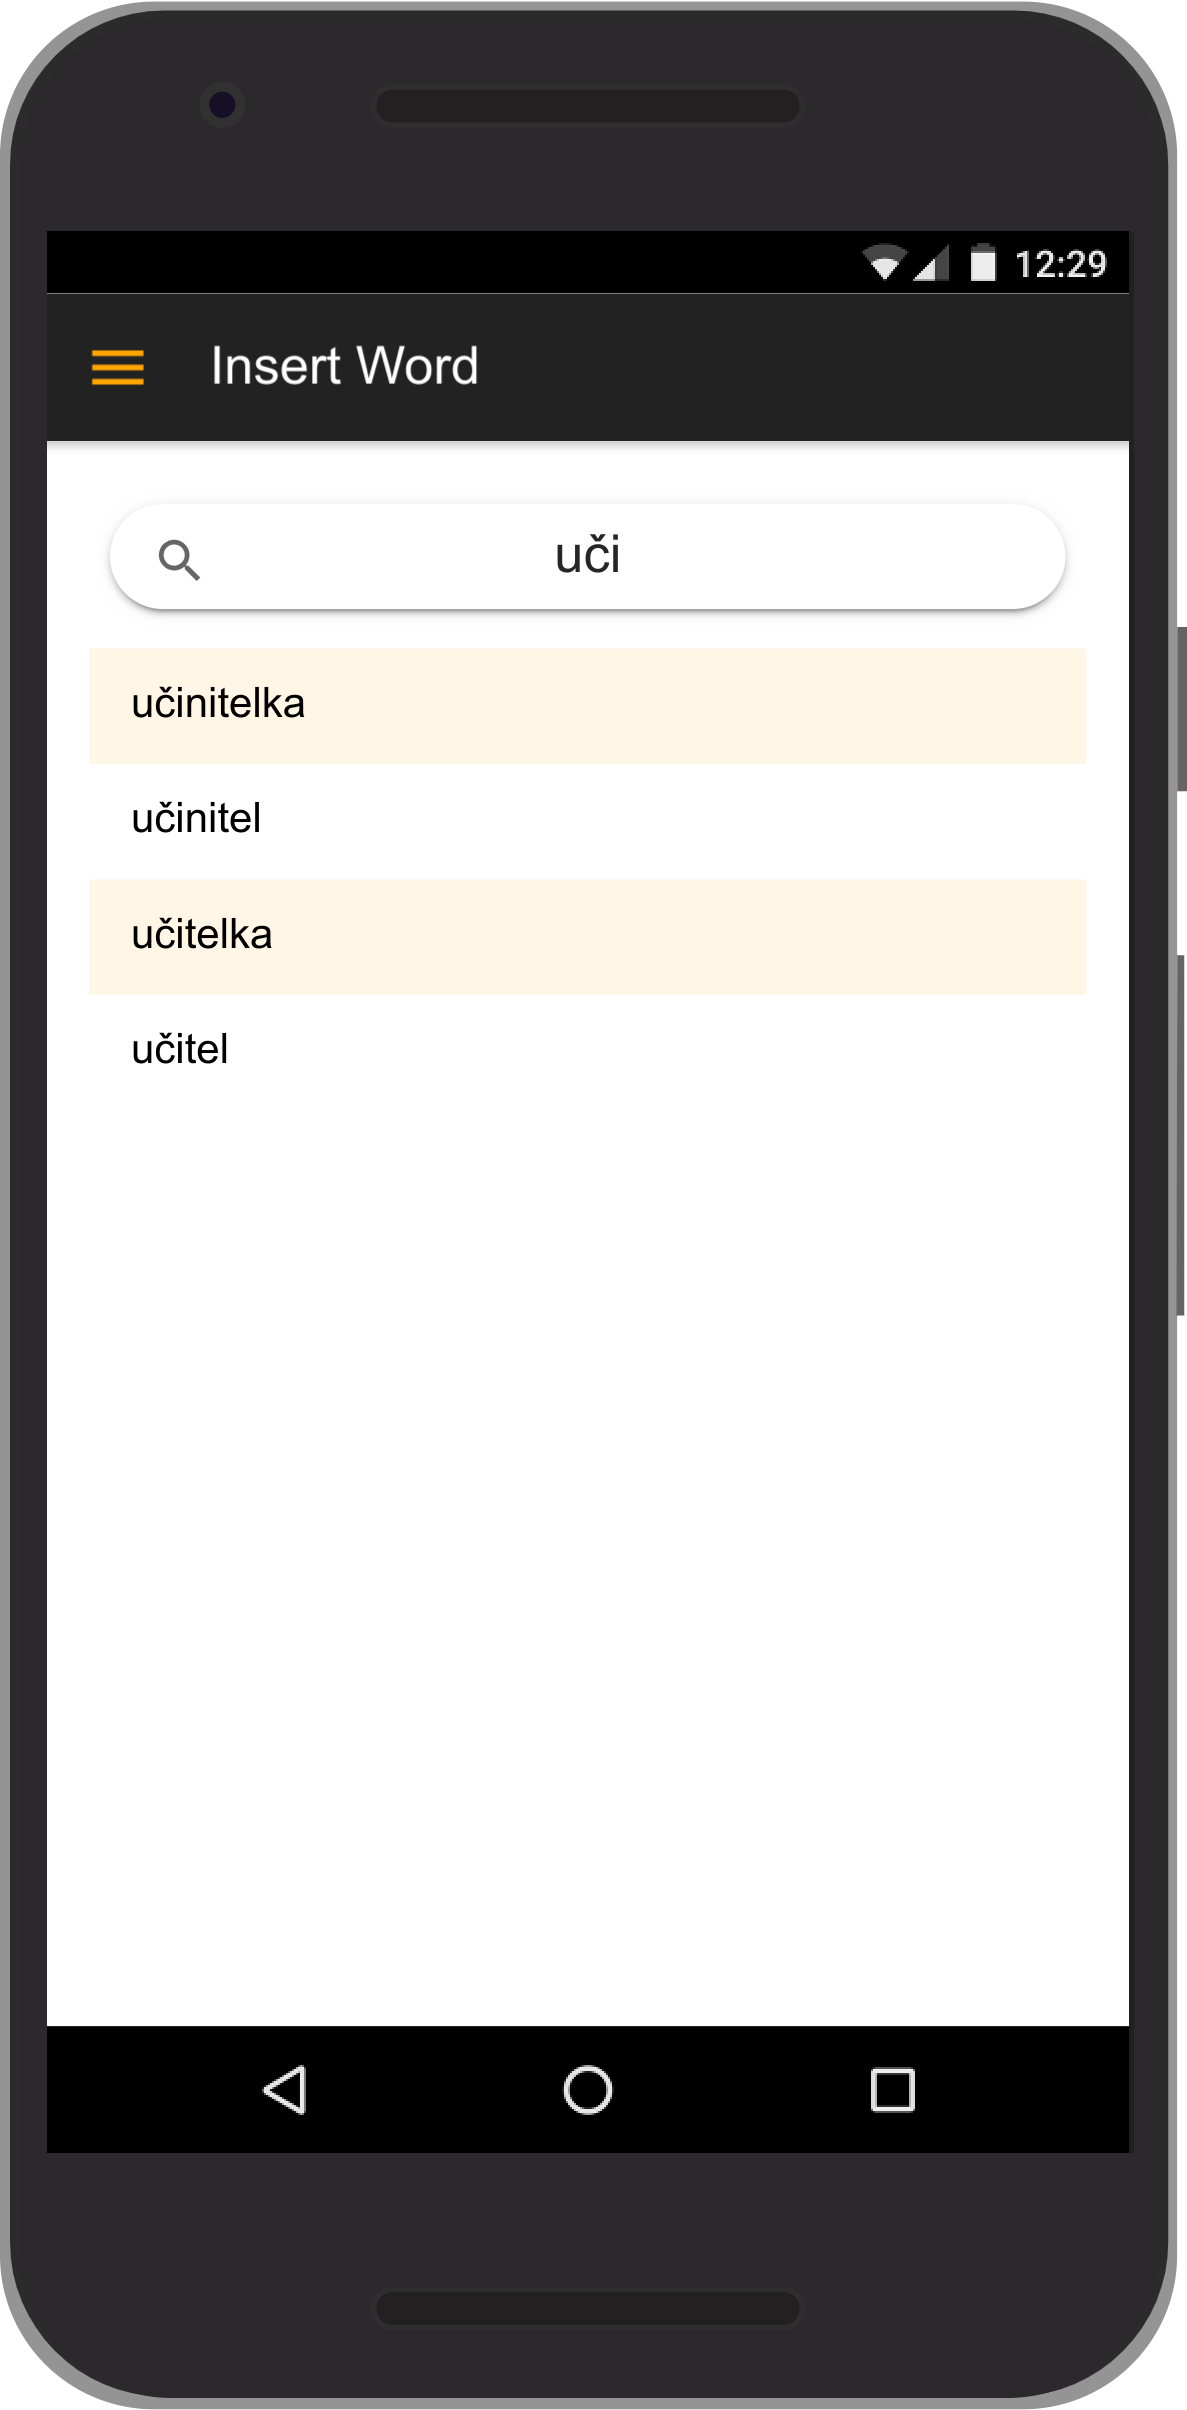
\includegraphics[width=\textwidth]{2-3}
  \end{subfigure}
  \caption{Proces zadávání vstupního slova}
  \label{2}
\end{figure}

Samotné slovníkové heslo je zobrazeno formou tří na sobě nezávislých
karet (viz obrázek \ref{3}), z~nichž každá obsahuje určité lingvistické
informace o~derivovaném výrazu (viz \ref{slovnuxedkovuxe9-heslo}).
V~případě, kdy je heslo vytvořeno na základě slova vybraného z~rejstříku
zpracovaných slov, může uživatel využít zobrazené navigační šipky (která
se zobrazí vedle vstupního výrazu po kliknutí na textové pole), jež ho
vrátí zpět na určité místo v~rejstříku.

\begin{figure}[ht]
  \begin{subfigure}[b]{0.45\textwidth}
    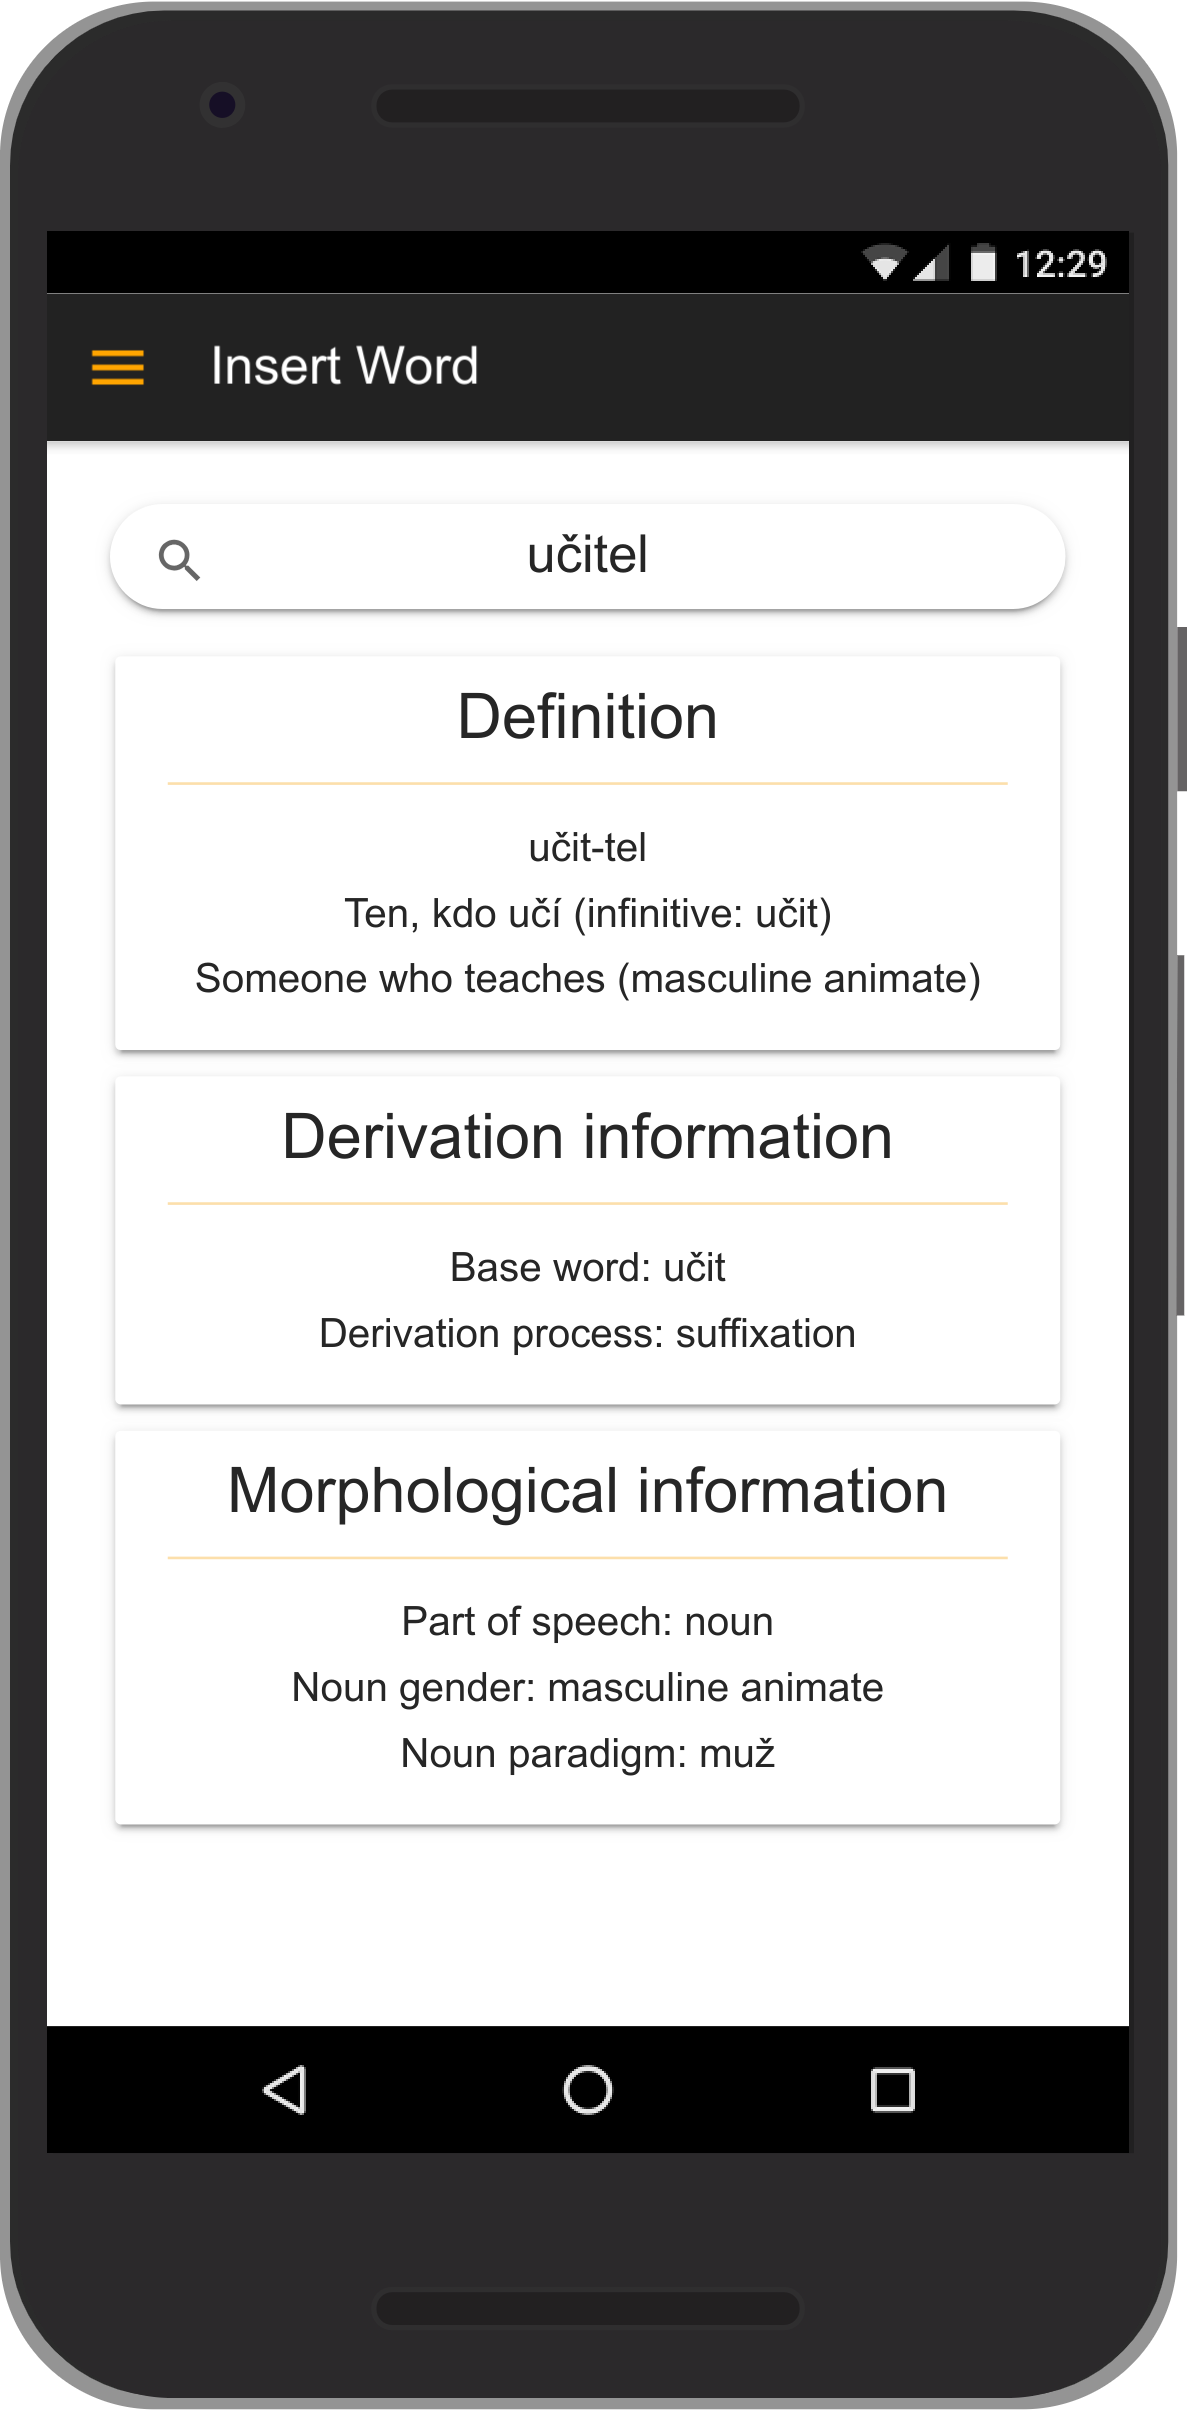
\includegraphics[width=0.9\textwidth]{3-1}
  \end{subfigure}
  \hfill
  \begin{subfigure}[b]{0.45\textwidth}
    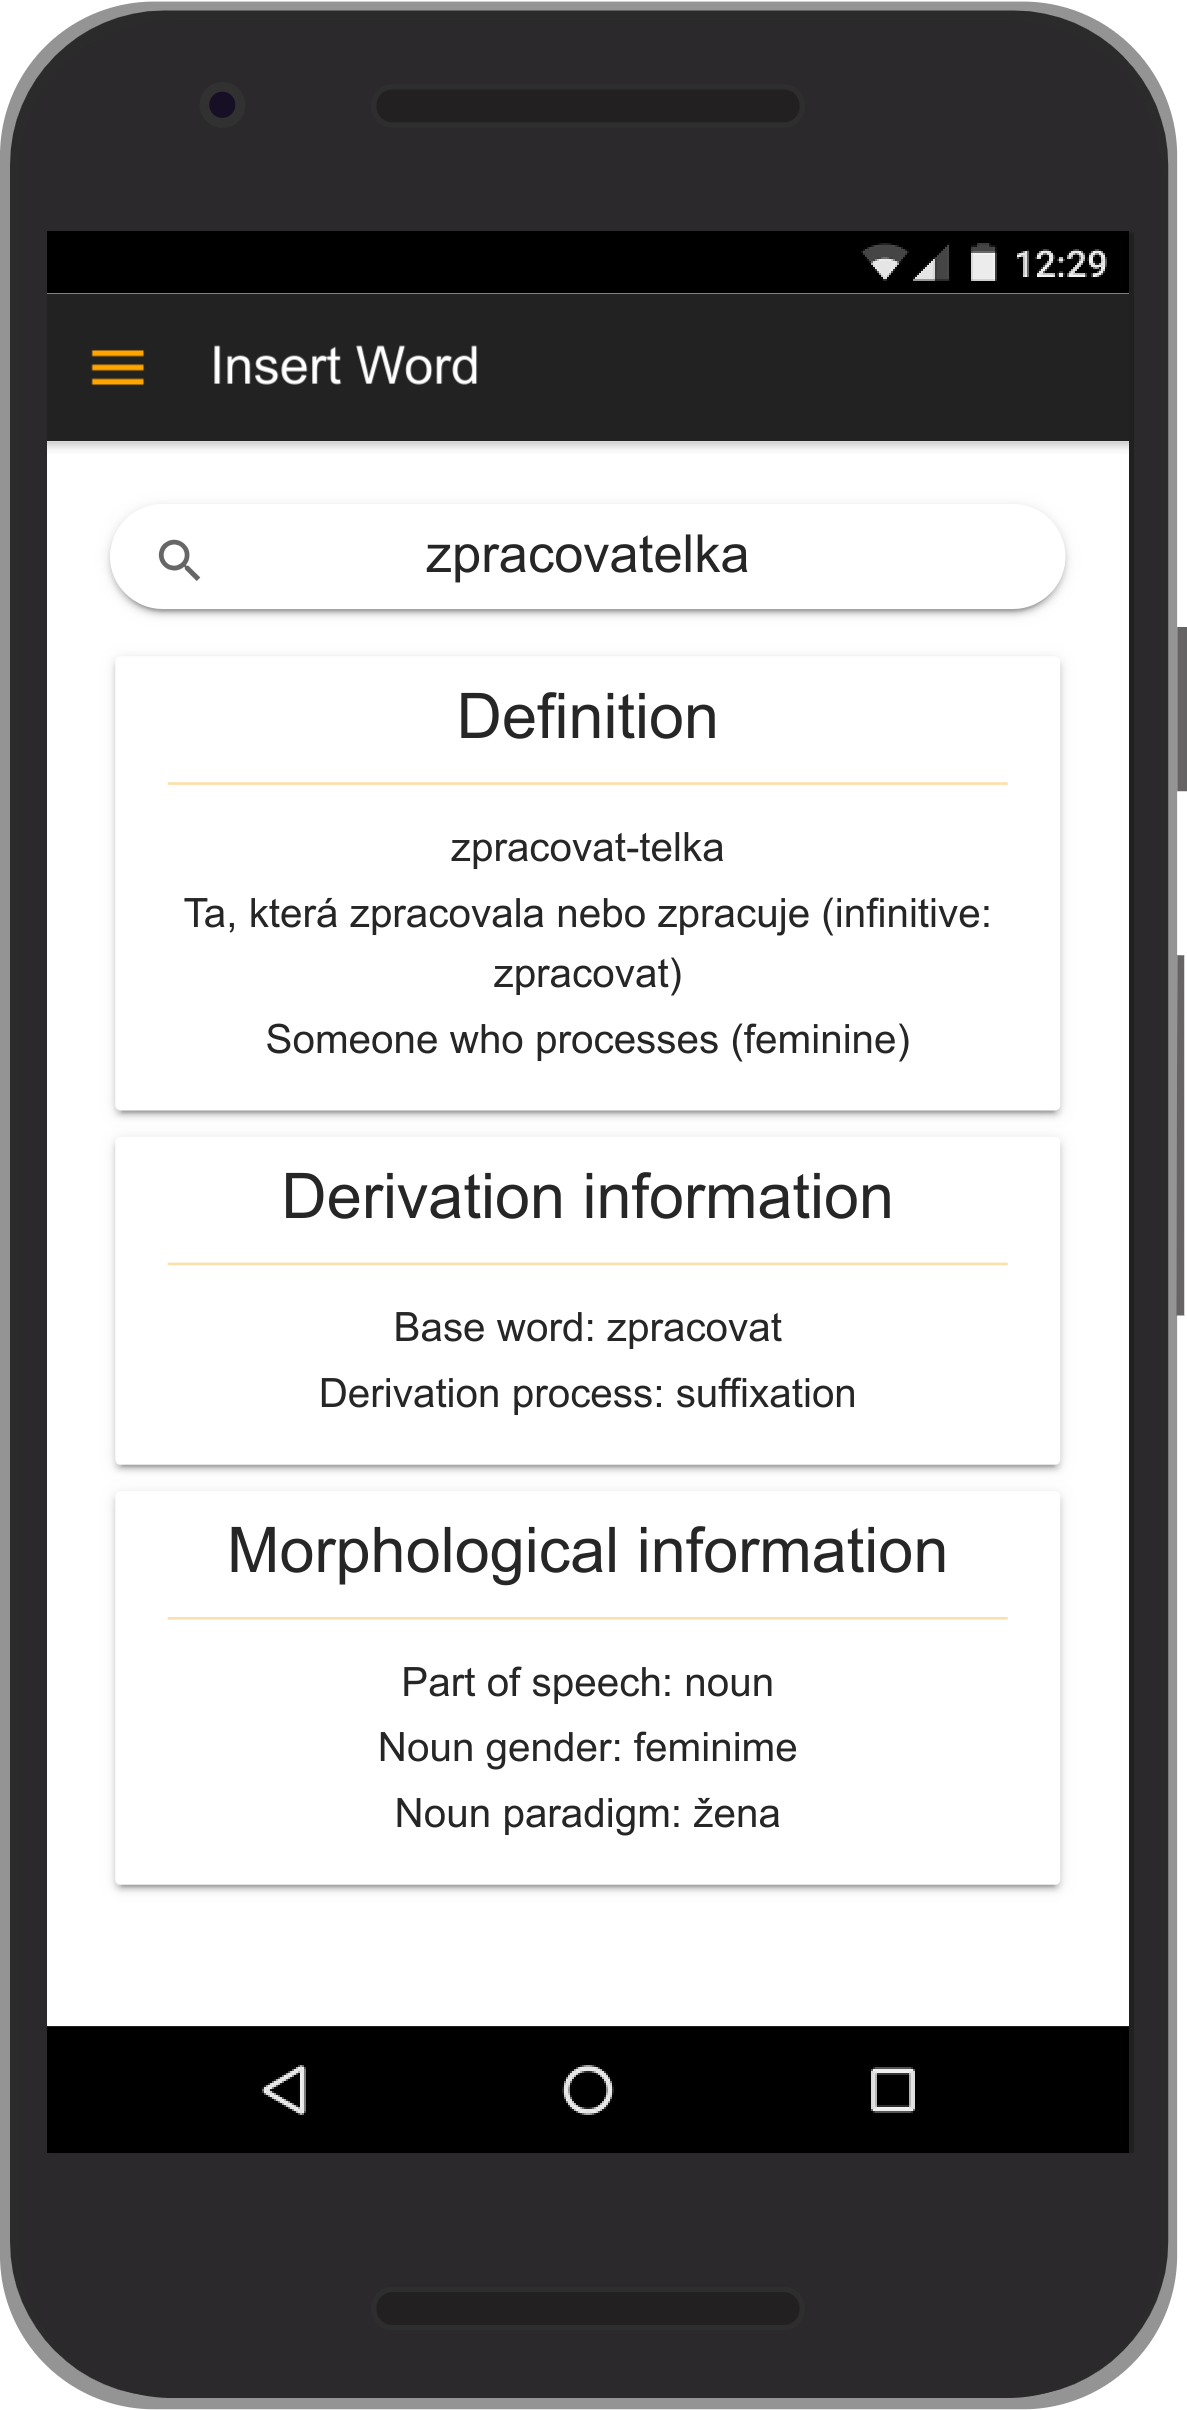
\includegraphics[width=0.9\textwidth]{3-2}
  \end{subfigure}
  \caption{Slovníková hesla}
  \label{3}
\end{figure}

Rejstřík zpracovaných slov je řazen abecedně a~obsahuje úplný seznam
slov (viz obrázek \ref{4}), která spadají do zpracovaných slovotvorných
typů. Jak bylo výše naznačeno, prostřednictvím rejstříku může uživatel
taktéž přistoupit k~vygenerování určitého slovníkového hesla.

Zbývají obrazovka je už jen marginální informační stránka týkající se
autorů, jež není pro popis návrhu uživatelského rozhraní nijak důležitá.

\begin{figure}[ht]
  \begin{subfigure}[b]{0.45\textwidth}
    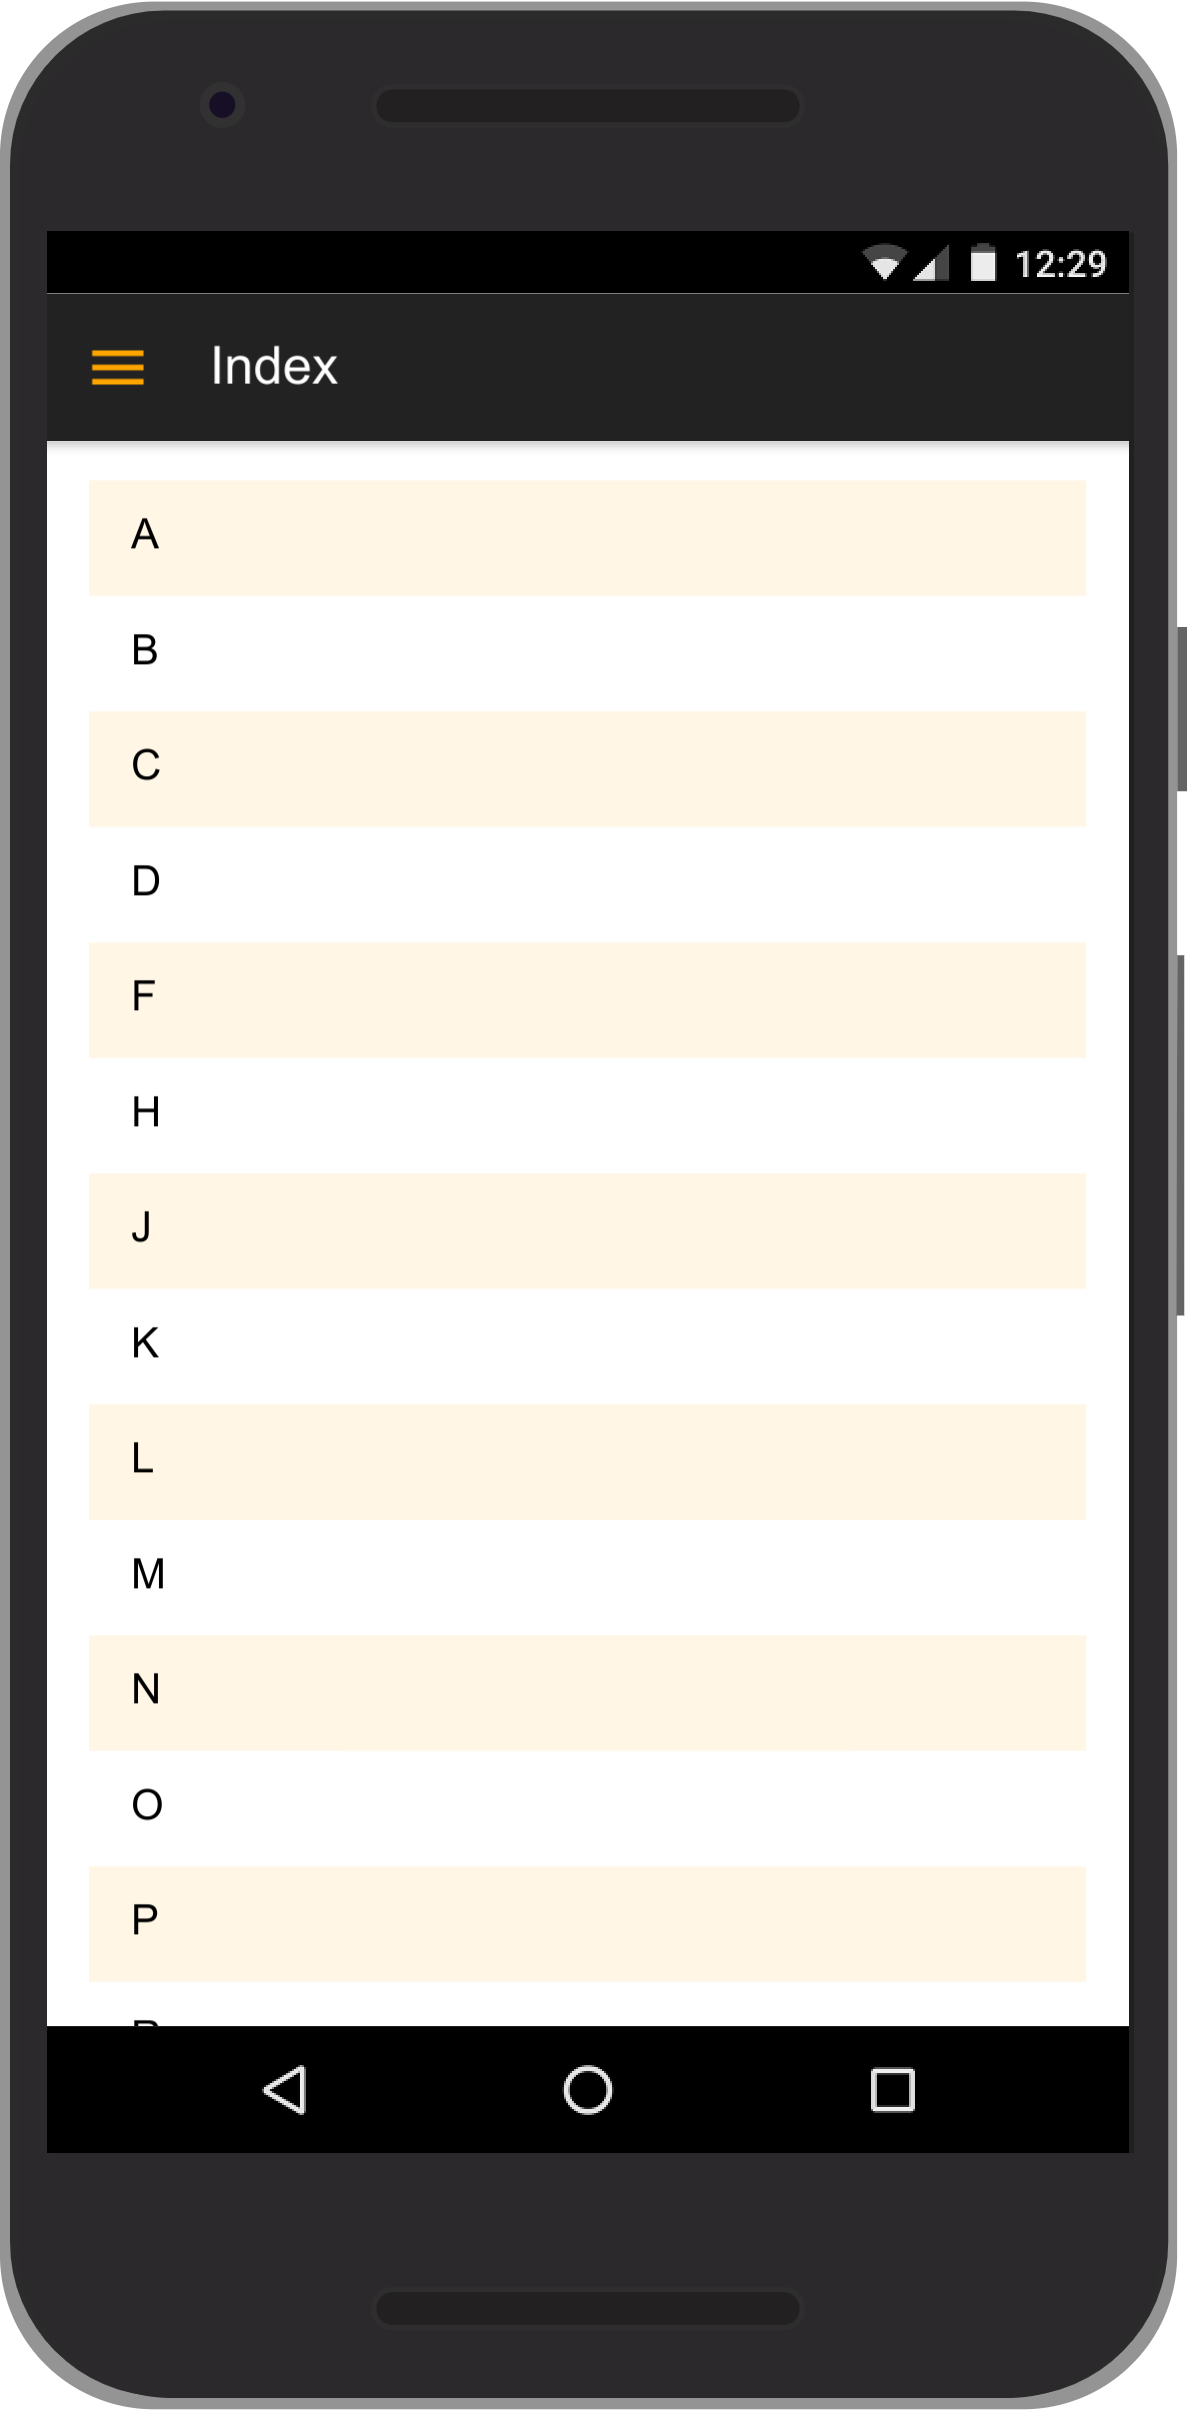
\includegraphics[width=0.9\textwidth]{4-1}
  \end{subfigure}
  \hfill
  \begin{subfigure}[b]{0.45\textwidth}
    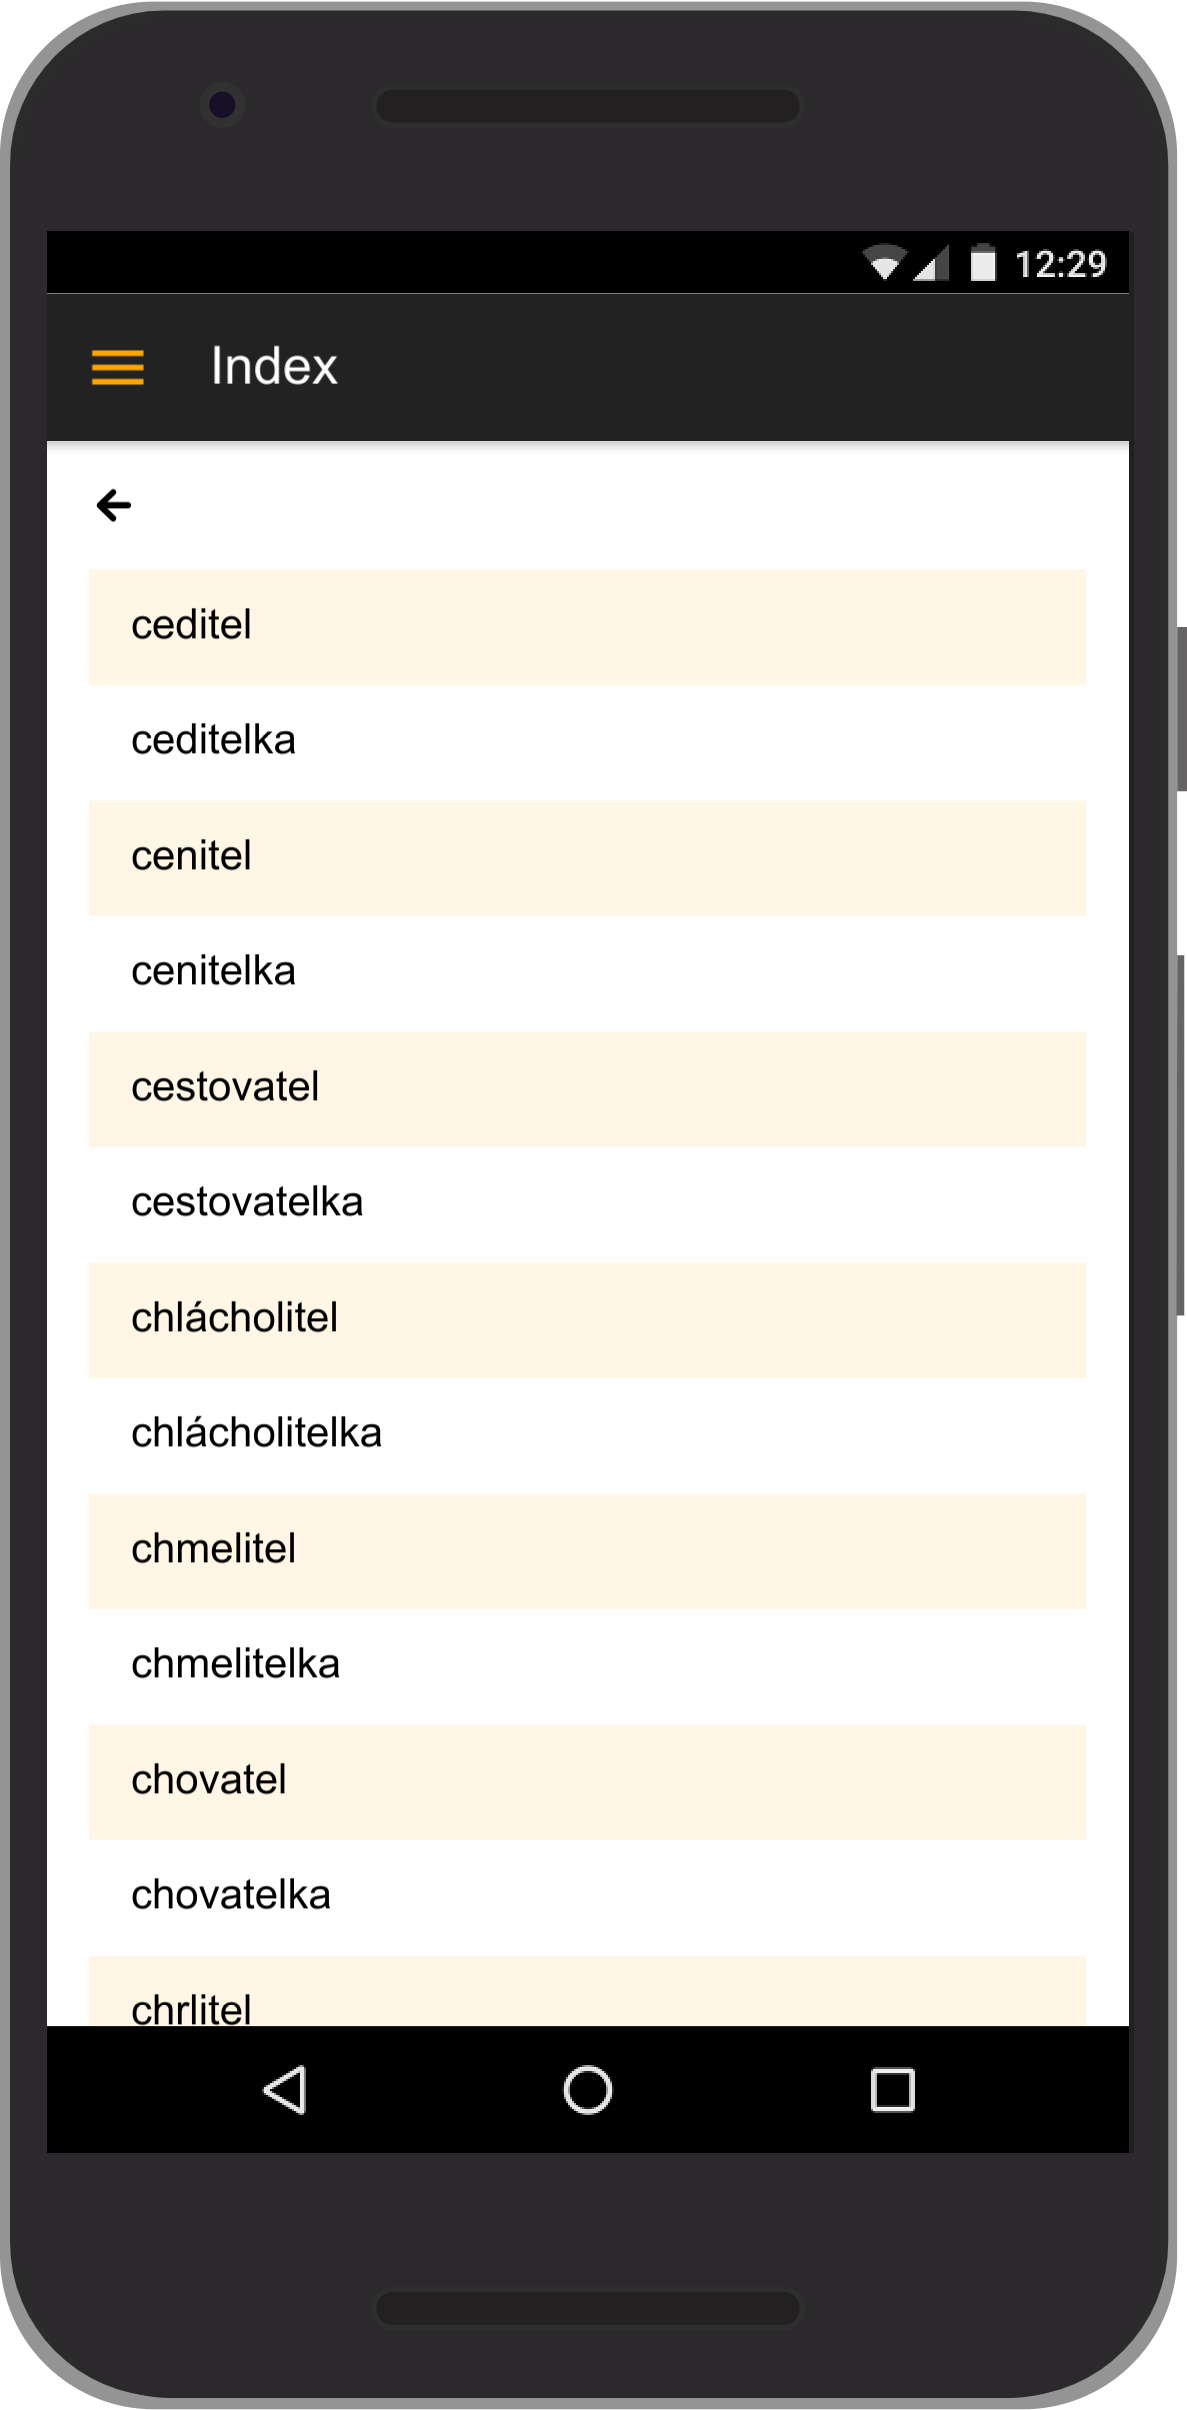
\includegraphics[width=0.9\textwidth]{4-2}
  \end{subfigure}
  \caption{Rejstřík zpracovaných slov}
  \label{4}
\end{figure}

\hypertarget{implementace-aplikace}{%
\section{Implementace aplikace}\label{implementace-aplikace}}

V~poslední kapitole si popíšeme architekturu předkládané aplikace spolu
s~její hlavní funkcionalitou \emph{insert word.}

\hypertarget{architektura}{%
\subsection*{Architektura aplikace}\label{architektura}}

Mobilní aplikace se skládá z~pěti hlavních stránek (komponent), jde o:

\begin{itemize}
\tightlist
\item
  vysouvací menu;
\item
  úvodní obrazovku s~informacemi o~aplikaci;
\item
  stránku s~funkcionalitou \emph{insert word};
\item
  rejstřík se zpracovanými slovy;
\item
  stránku s~informacemi o~autorech.
\end{itemize}

\hypertarget{insert word}{%
\subsection*{Alogritmus funkcionality insert word}\label{insert word}}

Implementačně nejkomplexnější je komponenta s~funkcionalitou
\emph{insert word}, proto se na ní v~následující části důkladněji
zaměříme a~pro demonstraci použitého algoritmu použijeme přiložené
schéma (viz obrázek \ref{algoritmus}). Pro větší přehlednost jsou na
diagramu modře zvýrazněny komponenty, žlutou barvou služby, zeleně
interní uložiště s~daty a~červeně pak hlavní funkce (ty se dále větví do
menších podfunkcí, jejichž popis není pro účely tohoto popisu klíčový).

\begin{figure}[ht]   
    \centering
    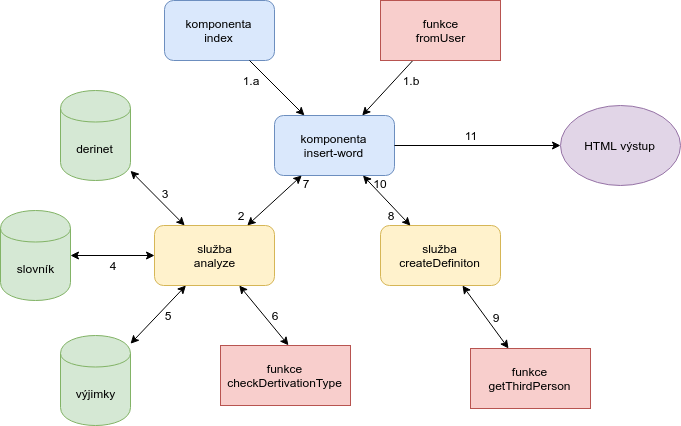
\includegraphics[width=.9\textwidth]{algoritmus}  
    \caption{Algoritmus funkcionality insert word}
    \label{algoritmus}
 \end{figure}

V~prvé řadě musí aplikace nějakým způsobem získat vstup pro následnou
analýzu, existují dva způsoby, jak k~tomu docílit. V~případě kroku 1.a
je za vstup považováno takové slovo, které bylo vybráno v~rámci
komponenty \emph{index}, tedy je vstupní slovo vybráno na stránce
s~rejstříkem zpracovaných slov. Druhou možností (1.b) je zadat slovo ručně
prostřednictvím funkce \emph{fromUser} z~textového pole, v~takovém
případě se po zadání prvního písmena (a~následně dalších znaků)
vyselektují všechna slova z~rejstříku, která začínají zadaným
podřetězcem.

V~okamžiku, kdy je vybráno vstupní slovo, je tento řetězec zaslán do
služby \emph{analyze} (2), která řeší všechny záležitosti týkající se
derivační sítě DeriNet a~překladu. V~této službě se při jejím volání
inicializuje objekt, který bude cílovým výstupem této služby -- tento
objekt nazýváme \emph{infoBase} a~skládá se z~několika atributů:

\begin{itemize}
\tightlist
\item
  vstup v~českém jazyce (při inicializaci je za jeho hodnotu přiřazeno
  vstupní slovo);
\item
  vstup v~anglickém jazyce (při inicializaci je spuštěn automatický
  překlad);
\item
  základové slovo v~českém jazyce (tento a~zbytek atributů zůstávají při
  inicializaci prázdné);
\item
  základové slovo v~anglickém jazyce;
\item
  slovotvorný typ;
\item
  prefigovanost;
\item
  prefix;
\item
  derivační proces;
\item
  rod;
\item
  derivační cesta.
\end{itemize}

Při inicializaci se souběžně načítají data z~interního uložiště, která
jsou následně zkonvertována do použitelného datového formátu (3, 4, 5),
konkrétně jde o~databázi DeriNet, česko-anglický slovník
Glosbe\footnote{https://glosbe.com/ -- jedná se o~open-source projekt pod licencí CC-BY-SA z~něhož byla vyextrahována data pro naše použití.}
a~seznam výjimek (viz kapitola
\ref{zpracovanuxe9-slovotvornuxe9-sufixy}).

Dalším krokem je postupné procházení derivační sítě DeriNet, z~níž
potřebujeme vyextrahovat výše zmíněné lingvistické informace, procházíme
tedy derivační řetězec směrem od slova vstupního k~jeho slovu
základovému do té chvíle, než se zamění slovní druh, pak přistupujeme
k~volání funkce \emph{checkDertivationType} (6). Ta nám porovná řetězce
obou slov a~určí, o~jaký se jedná derivační proces a~slovotvorný typ.
Dále určuje algoritmus z~celého derivačního řetězce prefigovanost
(popřípadě zjišťuje o~jaký prefix se přesně jedná), zaznamená si rod
vstupního slova (ve výjimkách máme tedy v~případě slovotvorného sufixu
\emph{-tel} taková slova, která jsou neživotnými maskuliny) a~ukládá si
základové slovo spolu s~jeho anglickým ekvivalentem (u~českých
odvozených slov ve slovníku často překlad chybí). Posléze služba
\emph{analyze} vrací již vyplněný objekt \emph{infoBase} zpátky do
komponenty \emph{insert-word}, vrácený objekt může vypadat například
takto:

\begin{verbatim}
1.  czechInput:  "zpracovatel"
2.  czechParent:  "zpracovat"
3.  derProcess:  "suffixation"
4.  derivType:  "tel"
5.  derivationPath:  (2) [{…},  {…}] // derivační řetězec
6.  englishInput:  ""
7.  englishParent:  "processes"
8.  gender:  "M"
9.  isPrefig:  true
10. prefix:  "z"
\end{verbatim}

Nyní se dostáváme do kroku č. 8, kdy je objekt \emph{infoBase} předán
druhé službě s~názvem \emph{createDefiniton}, jejímž účelem je vytvořit
samotné slovníkové heslo do formy objektu \emph{definiton}. Jednotlivé
části jsou zpracovány separátně, a~to jednak z~důvodu přehlednosti kódu,
ale taktéž z~ryze praktické příčiny, tedy aby s~výsledným objektem byla
co nejjednodušší manipulace na úrovní HTML šablony.

Na začátku inicializujeme obecnou slovotvornou definici podle rodu ze
vstupního objektu \emph{infoBase} a~poté přistupujeme k~funkci
\emph{getThirdPerson} (9), v~rámci které vytváříme slovesnou formu ve
třetí osobě podle lingvistických pravidel popsaných v~kapitole
\ref{slovotvornuxe1-definice}.

Následně dotvoříme derivační a~morfologickou informaci z~poznatků
získaných ze služby \emph{analyze} a~vracíme objekt \emph{definiton}
zpět do komponenty \emph{insert-word} (10). Pokud je vrácen objekt
správného typu, je HTML šabloně umožněno skrze direktivy frameworku
Angular přistoupit k~jednotlivým častém definice a~vykreslit je do
označených míst v~šabloně (11).

Výhoda tohoto objektového přístupu je taková, že se na jednotlivých
jasně otypovaných místech v~kódu provádí pouze jeden specifický úkol.
Tím je do určité míry zajištěna robustnost celkové aplikace, u~níž je
při výpadku jedné služby/funkce jednoduché lokalizovat místo chyby.

\hypertarget{zuxe1vux11br}{%
\chapter*{Závěr}\label{zaver}\addcontentsline{toc}{chapter}{Závěr}}

Cílem této bakalářské práce bylo navrhnout a~implementovat online kurz zaměřený na výuku základů datové analytiky. Kurz se podařilo vytvořit dle zadaných požadavků a~v~aktuální chvíli probíhá uživatelské testování v~rámci interních klientů firmy Digiskills, s~níž jsme návrh kurzu konzultovali. Jelikož získávání zpětné vazby na vytvořený online kurz stále probíhá, nelze v~tuto chvíli diskutovat výsledky testování, je nicméně pravděpodobné, že se některé části kurzu mohou na základě získaných odpovědí v~průběhu nejbližší doby mírně změnit .

Na vytvořený online kurz lze dále navázat několika různými způsoby. Jelikož se jedná o~úvodní vstup do problematiky, může být e-learning rozšířen o~pokročilejší témata týkající se složitějších statistických přístupů, které lze aplikovat na větší soubor dat (tedy částečně propojit datovou analytiku s~disciplínou data science). Další cestou může být komplexnější představení konkurenčních analytických nástrojů, s~nimiž se student může setkat napříč odlišnými organizacemi. Třetí možnost je akcentovat témata související s~vizualizací dat a~směřovat studenta spíše do oblasti business analytics, v~rámci které je důležitější efektivnější komunikace informací, nežli provádění náročnějších analýz.

Cíle této práce byly splněny a~její výstupy můžou být rozšířeny v~rámci případného navazujícího aplikovaného výzkumu týkající se uživatelského testování.

\clearpage

\pagestyle{plain}

\addcontentsline{toc}{chapter}{Seznam literatury}
\begin{spacing}{1.05}
\printbibliography[title={Seznam literatury}]
\end{spacing}

\end{document}